\documentclass[11pt]{article}

%{{{

\usepackage{october}
\usepackage{lineno}
% For BJPS
% \hyphenpenalty=10000
% \hbadness=10000

\begin{document}
\setpagewiselinenumbers
\modulolinenumbers[5]
\linenumbers
% For BJPS
% \raggedright
% \doublespacing

% y=3;z=4;pdftk A=epsa-jeffrey-conditioning\ \($y\).pdf cat A1-$z output wc-out.pdf

\title{Asymmetry and the Geometry of Reason}
\author{Stefan Lukits}
\date{}
\maketitle
% \newcounter{expls}
% \doublespacing

\begin{abstract}
  {\noindent}Defenders of the epistemic utility approach to Bayesian
  epistemology use the geometry of reason to justify Bayesian tenets
  such as probabilism and standard conditioning. The geometry of
  reason is the view that the underlying topology for credence
  functions is a metric space, on the basis of which axioms and
  theorems of epistemic utility for partial beliefs are formulated. It
  implies that Jeffrey conditioning must cede to an alternative form
  of conditioning. The latter fails a long list of plausible
  expectations. One solution to this problem is to reject the geometry
  of reason and accept information theory in its stead. Information
  theory comes fully equipped with an axiomatic approach which covers
  probabilism, standard conditioning, and Jeffrey conditioning. It is
  not based on an underlying topology of a metric space, but uses
  non-commutative divergences instead of a symmetric distance measure.
  I show that information theory, despite initial promise, also fails
  to accommodate basic epistemic intuitions.
% The paper, by
%   bringing the alternative of information theory to the forefront,
%   does therefore not clean up the mess but rather provides its
%   cartography.
\end{abstract}

\section{Introduction}
\label{intr}

In the early 1970s, the dominant models for similarity in the
psychological literature were all geometric in nature. Distance
measures capturing similarity and dissimilarity between concepts
obeyed minimality, symmetry, and the triangle inequality. Then Amos
Tversky wrote a compelling paper undermining the idea that a metric
topology is the best model (see \scite{7}{tversky77}{}). Tversky gave
both theoretical and empirical reasons why similarity between concepts
fulfills neither minimality, nor symmetry, nor the triangle inequality.
Geometry with its metric distance measures was in some ways not a
useful model of similarity. Tversky presented an alternative
set-theoretic account which accommodated intuitions that could not be
reconciled with a geometry of similarity.

The aim of this paper is to help along a similar paradigm shift when
it comes to epistemic modeling of closeness or difference between
subjective probability distributions. The \qnull{geometry of reason}
(a term coined by Richard Pettigrew and Hannes Leitgeb, two of its
advocates) violates reasonable expectations for an acceptable model. A
non-metric alternative, information theory, fulfills many of these
expectations but violates others which are similarly intuitive.
Instead of presenting a third alternative which coheres better with
the list of expectations outlined in section \ref{fivex}, I defend the
view that while the violations of the geometry of reason are
irremediable, there is a promise in the wings that an advanced formal
account of information theory, using the theory of differential
manifolds, can explain information theory's violations of prima facie
reasonable expectations.

The geometry of reason refers to a view of epistemic utility in which
the underlying topology for credence functions (which may be
subjective probability distributions) on a finite number of events is
a metric space. The set of non-negative credences that an agent
assigns to the outcome of a die roll, for example, is isomorphic to
$\mathbb{R}_{\geq{}0}^{6}$. If the agent fulfills the requirements of
probabilism, the isomorphism is to the more narrow set $\mathbb{S}^5$,
the five-dimensional simplex for which

\begin{equation}
  \label{eq:simplex}
  p_{1}+p_{2}+p_{3}+p_{4}+p_{5}+p_{6}=1.
\end{equation}

% There are several possibilities to deal with these violations: (i)
% reject both the geometry of reason and information theory and provide
% a third alternative; (ii) save one of the two accounts by weakening
% the expectations and giving plausible explanations for these
% weakenings, perhaps by providing a more advanced formal account; (iii)
% provide an impossibility theorem that shows that no model can fulfill
% all expectations. The last possibility would favour some sort of
% pluralism. I am not aware of a third alternative to the geometry of
% reason and information theory and personally favour possibility (ii).
% The model to save is information theory and the advanced formal
% account is the theory of differential manifolds. The problems for the
% geometry of reason are irremediable. This paper, however, only reveals
% the seriousness and extent of the violations, not the possible
% solutions.

For the remainder of this paper I will assume probabilism and an
isomorphism between probability distributions $P$ on an outcome space
$\Omega$ with $|\Omega|=n$ and points
$p\in\mathbb{S}^{n-1}\subset\mathbb{R}^{n}$ having coordinates
$p_{i}=P(\omega_{i}),i=1,\ldots,n$ and $\omega_{i}\in{}\Omega$. Since
the isomorphism is to a metric space, there is a distance relation
between credence functions which can be used to formulate axioms
relating credences to epistemic utility and to justify or to criticize
contentious positions such as Bayesian conditionalization, the
principle of indifference, other forms of conditioning, or probabilism
itself (see especially works cited below by James Joyce; Pettigrew and
Leitgeb; David Wallace and Hilary Greaves). For information theory, as
opposed to the geometry of reason, the underlying topology for
credence functions is not a metric space (see figures
\ref{fig:contourslp} and \ref{fig:contoursrj} for illustration).

\begin{figure}[ht]
  \begin{flushright}
    \begin{minipage}[h]{.7\linewidth}
      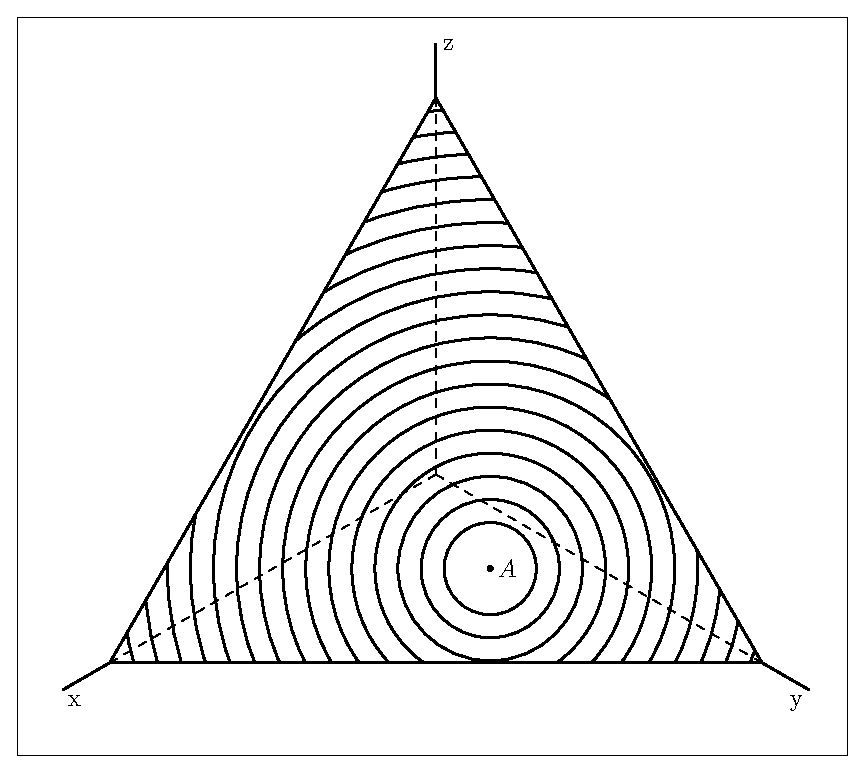
\includegraphics[width=\textwidth]{contourslp.eps}
      \caption{\footnotesize The simplex $\mathbb{S}^{2}$ in
        three-dimensional space $\mathbb{R}^{3}$ with contour lines
        corresponding to the geometry of reason around point $A$ in
        equation (\ref{eq:e6}). Points on the same contour line are
        equidistant from $A$ with respect to the Euclidean metric.
        Compare the contour lines here to figure
        \ref{fig:contoursrj}. Note that this diagram and all the
        following diagrams are frontal views of the simplex.}
      \label{fig:contourslp}
    \end{minipage}
  \end{flushright}
\end{figure}

\begin{figure}[ht]
  \begin{flushright}
    \begin{minipage}[h]{.7\linewidth}
      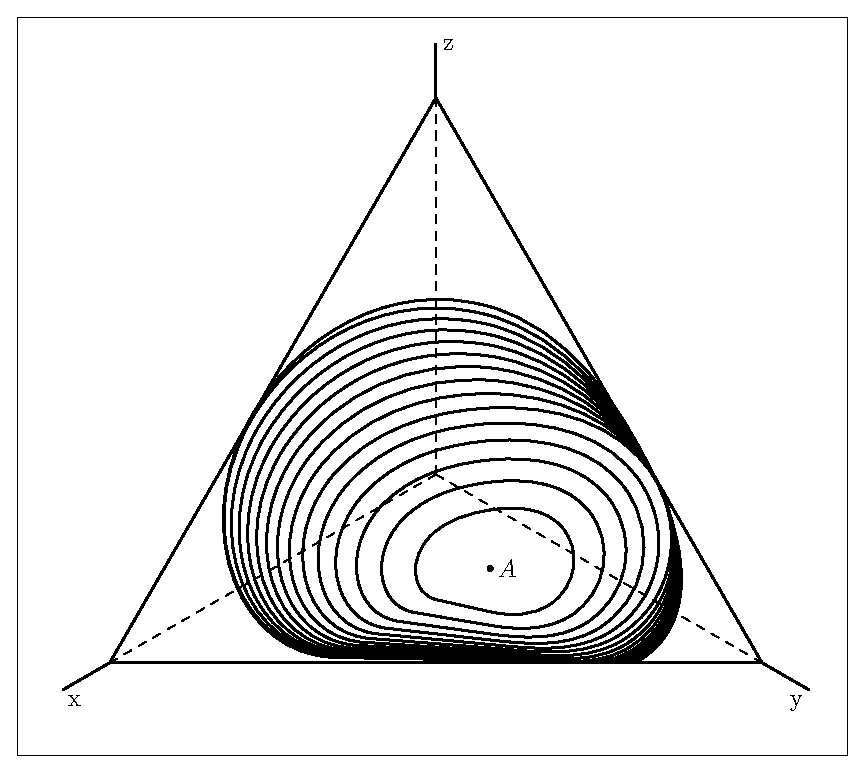
\includegraphics[width=\textwidth]{crj.eps}
      \caption{\footnotesize The simplex $\mathbb{S}^{2}$ with contour
        lines corresponding to information theory around point $A$ in
        equation (\ref{eq:e6}). Points on the same contour line are
        equidistant from $A$ with respect to the Kullback-Leibler
        divergence. The contrast to figure \ref{fig:contourslp} will
        become clear in much more detail in the body of the paper.
        Note that the contour lines of the geometry of reason are
        insensitive to the boundaries of the simplex, while the
        contour lines of information theory reflect them. One of the
        main arguments in this paper is that information theory
        respects epistemic intuitions we have about asymmetry:
        proximity to extreme beliefs with very high or very low
        probability influences the topology that is at the basis of
        updating.}
      \label{fig:contoursrj}
    \end{minipage}
  \end{flushright}
\end{figure}

Epistemic utility in Bayesian epistemology has attracted some
attention in the past few years. Patrick Maher provides a compelling
acceptance-based account of epistemic utility (see
\scite{8}{maher93}{182--207}). Joyce, in \qeins{A Nonpragmatic
  Vindication of Probabilism,} defends probabilism supported by
partial-belief-based epistemic utility rather than the pragmatic
utility common in Dutch-book style arguments (see
\scite{7}{joyce98}{}). For Joyce, norms of gradational accuracy
characterize the epistemic utility approach to partial beliefs,
analogous to norms of truth for full beliefs.

Wallace and Greaves investigate epistemic utility functions along
\qnull{stability} lines and conclude that for everywhere stable
utility functions standard conditioning is optimal, while only
somewhere stable utility functions create problems for maximizing
expected epistemic utility norms (see \scite{7}{greaveswallace06}{};
and \scite{7}{pettigrew13}{}). Richard Pettigrew and Hannes Leitgeb
have published arguments that under certain assumptions probabilism
and standard conditioning (which together give epistemology a distinct
Bayesian flavour) minimize inaccuracy, thereby providing maximal
epistemic utility (see Leitgeb and Pettigrew,
\scite{11}{leitgebpettigrew10i}{} and
\scite{11}{leitgebpettigrew10ii}{}).

Leitgeb and Pettigrew show, given the geometry of reason and other
axioms inspired by Joyce (for example normality and dominance), that
in order to avoid epistemic dilemmas we must commit ourselves to a
Brier score measure of inaccuracy and subsequently to probabilism and
standard conditioning. The Brier score is the mean squared error of a
probabilistic forecast. For example, if we look at 100 days for which
the forecast was 30\% rain and the incidence of rain was 32 days, then
the Brier score is
\begin{equation}
  \label{eq:thahthoo}
  \frac{1}{N}\sum_{t=1}^{N}\left(f_{t}-o_{t}\right)=\frac{1}{100}\left(32\cdot{}(0.3-1)+68\cdot{}(0.3-0)\right)=0.218
\end{equation}
$0$ is a perfect match between forecast and reality in the sense that
the forecaster anticipates every instance of rain with a 100\%
forecast and every instance of no rain with a 0\% forecast.

Jeffrey conditioning (also called probability kinematics) is widely
considered to be a commonsense extension of standard conditioning. On
Leitgeb and Pettigrew's account, using the Brier score, it fails to
provide maximal epistemic utility. Another type of conditioning, which
I will call LP conditioning, takes the place of Jeffrey conditioning.
The failure of Jeffrey conditioning to minimize inaccuracy on the
basis of the geometry of reason casts doubt on the geometry of reason
by reductio.

I will show that LP conditioning, which the geometry of reason
entails, fails commonsense expectations that are reasonable to have
for the kind of updating scenario that LP conditioning addresses. To
relate probability distributions to each other geometrically, using
the isomorphism between the set of probability distributions on a
finite event space $W$ with $|W|=n$ and the $n-1$-dimensional simplex
$\mathbb{S}^{n-1}\subset\mathbb{R}^{n}$, is initially an arbitrary
move. Leitgeb and Pettigrew do little to substantiate a link between
the geometry of reason and epistemic utility on a conceptual level. It
is the formal success of the model that makes the geometry of reason
attractive, but the failure of LP conditioning to meet basic
expectations undermines this success.

The question then remains whether we have a plausible candidate to
supplant the geometry of reason. The answer is yes: information theory
provides us with a measure of closeness between probability
distributions on a finite event space that has more conceptual appeal
than the geometry of reason, especially with respect to epistemic
utility---it is intuitively correct to relate coming-to-knowledge to
exchange of information. More persuasive than intuition, however, is
the fact that information theory supports both standard conditioning
(see \scite{7}{williams80}{}) and the extension of standard
conditioning to Jeffrey conditioning (see
\scite{7}{catichagiffin06}{}; and \scite{7}{lukits15}{}), an extension
which is on the one hand intuitive (see \scite{7}{wagner02}{})
and on the other hand formally continuous with the standard
conditioning which Leitgeb and Pettigrew have worked so hard to
vindicate nonpragmatically. LP conditioning is not continuous with
standard conditioning, which is reflected in one of the expectations
that LP conditioning fails to meet. 

\section{Epistemic Utility and the Geometry of Reason}
\label{eugr}

\subsection{Epistemic Utility for Partial Beliefs}
\label{subsec:oochihei}

There is more epistemic utility for an agent in believing a truth
rather than not believing it and in not believing a falsehood rather
than believing it. Accuracy in full belief epistemology can be
measured by counting four sets, believed truths and falsehoods as well
as unbelieved truths and falsehoods, and somehow relating them to each
other such that epistemic utility is rewarded and epistemic vice
penalized. Accuracy in partial belief epistemology must take a
different shape since as a \qnull{guess} all partial non-full beliefs
are off the mark so that they need to be appreciated as
\qnull{estimates} instead. Richard Jeffrey distinguishes between
guesses and estimates: a guess fails unless it is on target, whereas
an estimate succeeds depending on how close it is to the target.

The gradational accuracy needed for partial belief epistemology is
reminiscent of verisimilitude and its associated difficulties in the
philosophy of science (see \scite{7}{popper63}{};
\scite{7}{gemes07}{}; and \scite{7}{oddie13}{}). Joyce and
Leitgeb/Pettigrew propose various axioms for a measure of gradational
accuracy for partial beliefs relying on the geometry of reason, i.e.\
the idea of geometrical distance between distributions of partial
belief expressed in non-negative real numbers. In Joyce, a metric
space for probability distributions is adopted without much
reflection. The midpoint between two points, for example, which is
freely used by Joyce, assumes symmetry between the end points. The
asymmetric divergence measure that I propose as an alternative to the
Euclidean distance measure has no meaningful concept of a midpoint.

Leitgeb and Pettigrew muse about alternative geometries, especially
non-Euclidean ones. They suspect that these would be based on and in
the end reducible to Euclidean geometry but they do not entertain the
idea that they could drop the requirement of a metric topology
altogether (for the use of non-Euclidean geodesics in statistical
inference see \scite{7}{amari85}{}). Thomas Mormann explicitly warns
against the assumption that the metrics for a geometry of logic is
Euclidean by default: \qeins{All too often, we rely on geometric
  intuitions that are determined by Euclidean prejudices. The geometry
  of logic, however, does not fit the standard Euclidean metrical
  framework} (see \scite{8}{mormann05}{433}; also
\scite{7}{miller84}{}). Mormann concludes in his article
\qeins{Geometry of Logic and Truth Approximation,}

\begin{quotex}
  Logical structures come along with ready-made geometric structures
  that can be used for matters of truth approximation. Admittedly,
  these geometric structures differ from those we are accostumed [sic]
  with, namely, Euclidean ones. Hence, the geometry of logic is not
  Euclidean geometry. This result should not come as a big surprise.
  There is no reason to assume that the conceptual spaces we use for
  representing our theories and their relations have an [sic]
  Euclidean structure. On the contrary, this would appear to be an
  improbable coincidence. \scite{3}{mormann05}{453}
\end{quotex}

\subsection{Axioms for Epistemic Utility}
\label{subsec:eichaequ}

Leitgeb and Pettigrew present the following salient axioms (see
\scite{8}{leitgebpettigrew10i}{219}):

\begin{quotex}
  \textbf{Local Normality and Dominance}: If $I$ is a legitimate
  inaccuracy measure, then there is a strictly increasing function
  $f:\mathbb{R}^{+}_{0}\rightarrow\mathbb{R}^{+}_{0}$ such that, for
  any $A\in{}W$, $w\in{}W$, and $x\in\mathbb{R}^{+}_{0}$,
  \begin{equation}
    \label{eq:e4}
    I(A,w,x)=f\left(|\chi_{A}(w)-x|\right).
  \end{equation}
\end{quotex}

\begin{quotex}
  \textbf{Global Normality and Dominance}: If $G$ is a legitimate
  global inaccuracy measure, there is a strictly increasing function
  $g:\mathbb{R}^{+}_{0}\rightarrow\mathbb{R}^{+}_{0}$ such that, for
  all worlds $w$ and belief functions $b\in{}\mbox{Bel}(W)$,
  \begin{equation}
    \label{eq:e5}
  G(w,b)=g\left(\|w-b_{\mbox{{\tiny glo}}}\|\right).
  \end{equation}
\end{quotex}

Similarly to Joyce, these axioms are justified on the basis of
geometry, but this time more explicitly so:

\begin{quotex}
  Normality and Dominance [are] a consequence of taking seriously the
  talk of inaccuracy as \qnull{distance} from the truth, and [they
  endorse] the geometrical picture provided by Euclidean $n$-space as
  the correct clarification of this notion. As explained in section
  3.2, the assumption of this geometrical picture is one of the
  presuppositions of our account, and we do not have much to offer in
  its defense, except for stressing that we would be equally
  interested in studying the consequences of minimizing expected
  inaccuracy in a non-Euclidean framework. But without a doubt,
  starting with the Euclidean case is a natural thing to do.
\end{quotex}

Leitgeb and Pettigrew define two notions, local and global inaccuracy,
and show that one must adopt a Brier score to measure inaccuracy in
order to avoid epistemic dilemmas trying to minimize inaccuracy on
both measures. To give the reader an idea what this looks like in
detail and for purposes of later exposition, I want to provide some of
the formal apparatus. Let $W$ be a set of worlds and $A\subseteq{}W$ a
proposition. Then

\begin{equation}
  \label{eq:linacc}
  I:P(W)\times{}W\times{}\mathbb{R}^{+}_{0}\rightarrow\mathbb{R}^{+}_{0}
\end{equation}

{\noindent}is a measure of local inaccuracy such that $I(A,w,x)$
measures the inaccuracy of the degree of credence $x$ with respect to
$A$ at world $w$. Let $\mbox{Bel}(W)$ be the set of all belief
functions (what I have been calling distributions of partial belief).
Then

\begin{equation}
  \label{eq:ginacc}
  G:W\times\mbox{Bel}(W)\rightarrow\mathbb{R}^{+}_{0}
\end{equation}

{\noindent}is a measure of global inaccuracy of a belief function $b$
at a possible world $w$ such that $G(w,b)$ measures the inaccuracy of
a belief function $b$ at world $w$.

Axioms such as normality and dominance guarantee that the only
legitimate measures of inaccuracy are Brier scores if one wants to
avoid epistemic dilemmas where one receives conflicting advice from
the local and the global measures. For local inaccuracy measures, this
means that there is $\lambda\in\mathbb{R}^{+}$ such that

\begin{equation}
  \label{eq:e1}
  I(A,w,x)=\lambda\left(\chi_{A}(w)-x\right)^{2}
\end{equation}

where $\chi_{A}$ is the characteristic function of $A$. For global
inaccuracy measures, this means that there is $\mu\in\mathbb{R}^{+}$
such that

\begin{equation}
  \label{eq:e2}
  G(w,b)=\mu\|w-b\|^{2}
\end{equation}

where $w$ and $b$ are represented by vectors and $\|u-v\|$ is the
Euclidean distance

\begin{equation}
  \label{eq:e3}
  \sqrt{\sum_{i=1}^{n}\left(u_{i}-v_{i}\right)^{2}}.
\end{equation}

We use (\ref{eq:e1}) to define expected local inaccuracy of degree of
belief $x$ in proposition $A$ by the lights of belief function $b$,
with respect to local inaccuracy measure $I$, and over the set $E$ of
epistemically possible worlds as follows:

\begin{equation}
  \label{eq:eli}
  \mbox{LExp}_{b}(I,A,E,x)=\sum_{w\in{}E}b(\{w\})I(A,w,x)=\sum_{w\in{}E}b(\{w\})\lambda\left(\chi_{A}(w)-x\right)^{2}.
\end{equation}

We use (\ref{eq:e2}) to define expected global inaccuracy of belief
function $b'$ by the lights of belief function $b$, with respect to
global inaccuracy measure $G$, and over the set $E$ of epistemically
possible worlds as follows:

\begin{equation}
  \label{eq:egi}
  \mbox{GExp}_{b}(G,E,b')=\sum_{w\in{}E}b(\{w\})G(w,b')=\sum_{w\in{}E}b(\{w\})\mu\|w-b\|^{2}.
\end{equation}

To give a flavour of how attached the axioms are to the geometry of
reason, here are Joyce's axioms called Weak Convexity and Symmetry,
which he uses to justify probabilism. Note that in terms of notation
$I$ for Joyce is global and related to Leitgeb and Pettigrew's $G$ in
(\ref{eq:ginacc}) rather than $I$ in (\ref{eq:linacc}).

\begin{quotex}
\label{quot:weakconv}
  \textbf{Weak Convexity}: Let $m=(0.5b'+0.5b'')$ be the midpoint of the line
  segment between $b'$ and $b''$. If $I(b',\omega)=I(b'',\omega)$,
  then it will always be the case that $I(b',\omega)\geq{}I(m,\omega)$
  with identity only if $b'=b''$.
\end{quotex}

\begin{quotex}
\label{quot:symmetry}
  \textbf{Symmetry}: If $I(b',\omega)=I(b'',\omega)$, then for any
  $\lambda\in{}[0,1]$ one has\newline
  $I(\lambda{}b'+(1-\lambda)b'',\omega)=I((1-\lambda){}b'+\lambda{}b''),\omega)$.
\end{quotex}

Joyce advocates for these axioms in Euclidean terms, using
justifications such as \qeins{the change in belief involved in going
  from $b'$ to $b''$ has the same direction but a doubly greater
  magnitude than change involved in going from $b'$ to [the midpoint]
  $m$} (see \scite{8}{joyce98}{596}). In section
\ref{subsec:Asymmetry}, I will show that Weak Convexity holds, and
Symmetry does not hold, in \qnull{information geometry,} the topology
generated by the Kullback-Leibler divergence. The term information
geometry is due to Imre Csisz{\'a}r, who considers the
Kullback-Leibler divergence a non-commutative (asymmetric) analogue of
squared Euclidean distance and derives several results that are
intuitive information geometric counterparts of standard results in
Euclidean geometry (see chapter 3 of \scite{7}{csiszarshields04}{}).

\subsection{Expectations for Jeffrey-Type Updating Scenarios}
\label{subsec:vidiedoo}

Leitgeb and Pettigrew's work is continuous with Joyce's work, but
significantly goes beyond it. Joyce wants weaker assumptions and would
be leery of expected inaccuracies (\ref{eq:eli}) and (\ref{eq:egi}),
as they might presuppose the probabilism that Joyce wants to justify.
Leitgeb and Pettigrew investigate not only whether probabilism and
standard conditioning follow from gradational accuracy based on the
geometry of reason, but also uniform distribution (their term for the
claim of objective Bayesians that there is some principle of
indifference for ignorance priors) and Jeffrey conditioning. They show
that uniform distribution requires additional axioms which are much
less plausible than the ones on the basis of which they derive
probabilism and standard conditioning (see
\scite{8}{leitgebpettigrew10ii}{250f}); and that Jeffrey conditioning
does not fulfill Joyce's Norm of Gradational Accuracy (see
\scite{8}{joyce98}{579}) and therefore violates the pursuit of
epistemic utility. Leitgeb and Pettigrew provide us with an alternative
method of updating for Jeffrey-type updating scenarios, which I will
call LP conditioning.

\begin{quotex}
  \beispiel{Sherlock Holmes}\label{ex:holmes} Sherlock Holmes
  attributes the following probabilities to the propositions $E_{i}$
  that $k_{i}$ is the culprit in a crime:
  $P(E_{1})=1/3,P(E_{2})=1/2,P(E_{3})=1/6$, where $k_{1}$ is Mr.\ R.,
  $k_{2}$ is Ms.\ S., and $k_{3}$ is Ms.\ T. Then Holmes finds some
  evidence which convinces him that $P'(F^{*})=1/2$, where $F^{*}$ is
  the proposition that the culprit is male and $P$ is relatively prior
  to $P'$. What should be Holmes' updated probability that Ms.\ S. is
  the culprit?
\end{quotex}

% toodeloo
I will look at the recommendations of Jeffrey conditioning and LP
conditioning for {\xample} \ref{ex:holmes} in the next section. For
now note that LP conditioning violates all of the following plausible
expectations in \textbf{List A}\label{page:listone} for an amujus, 
short for \qnull{a method of updating for Jeffrey-type updating
  scenarios.} This is \textbf{List A}:

\begin{itemize}
\item \textsc{continuity} An amujus ought to be continuous with
  standard conditioning as a limiting case.
\item \textsc{regularity} An amujus ought not to assign a posterior
  probability of $0$ to an event which has a positive prior
  probability and about which the intervening evidence says nothing
  except that a strictly weaker event has a positive posterior
  probability.
\item \textsc{levinstein} An amujus ought not to give \qeins{extremely
    unattractive} results in a Levinstein scenario (see
  \scite{7}{levinstein12}{}, which not only articulates this failed
  expectation for LP conditioning, but also the previous two).
\item \textsc{invariance} An amujus ought to be partition invariant.
\item \textsc{expansibility} An amujus ought to be insensitive to an
  expansion of the event space by zero-probability events.
\item \textsc{confirmation} An amujus ought to align with intuitions
  we have about degrees of confirmation.
\item \textsc{horizon} An amujus ought to exhibit the horizon effect
  which makes probability distributions which are nearer to extreme
  probability distributions appear to be closer to each other than
  they really are.
\end{itemize}

Jeffrey conditioning and LP conditioning are both an amujus based on a
concept of quantitative difference between probability distributions
measured as a function on the isomorphic manifold (in our case, an
$n-1$-dimensional simplex). Evidence appears in the form of a
constraint on acceptable probability distributions and the closest
acceptable probability to the orginal (relatively prior) probability
distribution is chosen as its successor. Here is \textbf{List
  B}\label{page:listtwo}, a list of reasonable expectations one may
have toward this concept of quantitative difference (we call it a
distance function for the geometry of reason and a divergence for
information theory). Let $d(p,q)$ express this concept mathematically.

\begin{itemize}
\item \textsc{triangularity} The concept obeys the triangle
  inequality. If there is an intermediate probability distribution, it
  will not make the difference smaller: $d(p,r)\leq{}d(p,q)+d(q,r)$.
  Buying a pair of shoes is not going to be more expensive than buying
  the two shoes individually.
\item \textsc{collinear horizon} This expecation is just a more
  technical restatement of the \textsc{horizon} expectation in the
  previous list. If $p,p',q,q'$ are collinear with the centre of the
  simplex $m$ (whose coordinates are $m_{i}=1/n$ for all $i$) and an
  arbitrary but fixed boundary point $\xi\in\partial\mathbb{S}^{n-1}$
  and $p,p',q,q'$ are all between $m$ and $\xi$ with
  $\|p'-p\|=\|q'-q\|$ where $p$ is strictly closest to $m$, then
  $|d(p,p')|<|d(q,q')|$. For an illustration of this expectation see
  figure \ref{fig:conditions}. The absolute value is added as a
  feature to accommodate degree of confirmation functions in
  subsection \ref{Confirmation}, which may be negative.
\item \textsc{transitivity of asymmetry} An ordered pair $(p,q)$ of
  simplex points associated with probability distributions is
  asymmetrically negative, positive, or balanced, so either
  $d(p,q)-d(q,p)<0$ or $d(p,q)-d(q,p)>0$ or $d(p,q)-d(q,p)=0$. If
  $(p,q)$ and $(q,r)$ are asymmetrically positive, $(p,r)$ ought not
  to be asymmetrically negative. Think of a bicycle route map with
  different locations at varying altitudes. If it takes 20 minutes to
  get from $A$ to $B$ but only 15 minutes to get from $B$ to $A$ then
  $(A,B)$ is asymmetrically positive. If $(A,B)$ and $(B,C)$ are
  asymmetrically positive, then $(A,C)$ ought not to be asymmetrically
  negative.
\end{itemize}

\begin{figure}[ht]
  \begin{flushright}
    \begin{minipage}[h]{.7\linewidth}
      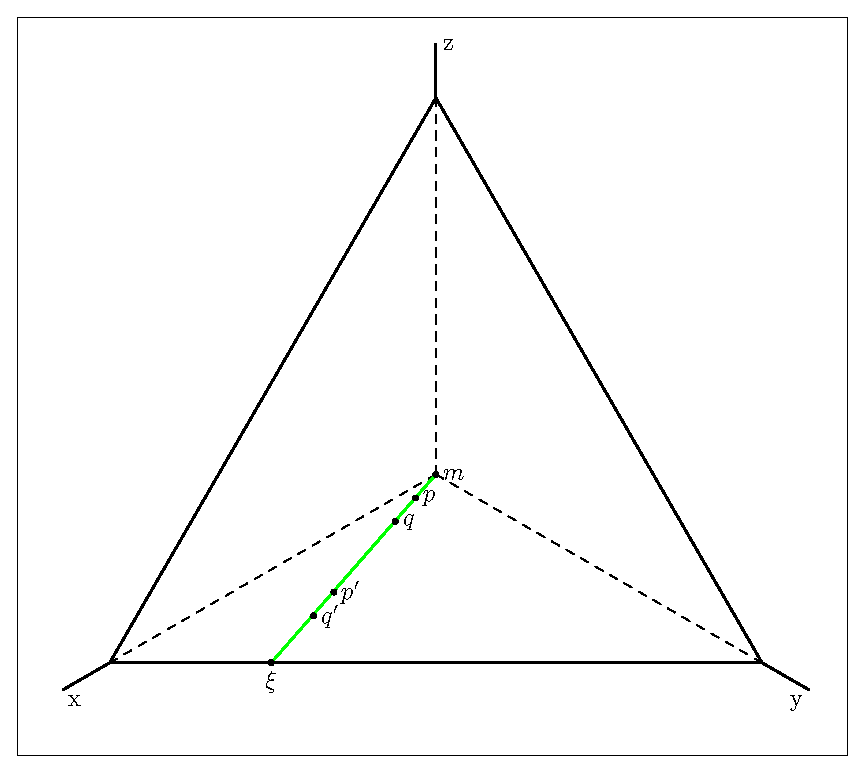
\includegraphics[width=\textwidth]{horeff.eps}
      \caption{\footnotesize An illustrations of conditions (i)--(iii)
        for \textsc{collinear horizon} in \textbf{List B}. $p,p'$ and $q,q'$
        must be equidistant and collinear with $m$ and $\xi$. If
        $q,q'$ is more peripheral than $p,p'$, then \textsc{collinear
          horizon} requires that $|d(p,p')|<|d(q,q')|$.}
      \label{fig:conditions}
    \end{minipage}
  \end{flushright}
\end{figure}

While the Kullback-Leibler divergence of information theory fulfills
all the expectations of \textbf{List A}, save \textsc{horizon}, it fails all
the expectations in \textbf{List B}. Obversely, the Euclidean distance of the
geometry of reason fulfills all the expectations of \textbf{List B}, save
\textsc{collinear horizon}, and fails all the expectations in \textbf{List A}. Information theory has its own axiomatic approach to justifying
probabilism and standard conditioning (see
\scite{7}{shorejohnson80}{}). Information theory provides a
justification for Jeffrey conditioning and generalizes it (see
\scite{7}{lukits15}{}). All of these virtues stand in contrast to the
violations of the expectations in \textbf{List B}. The rest of this paper
fills in the details of these violations both for the geometry of
reason and information theory, with the conclusion that the case for
the geometry of reason is hopeless while the case for information
theory is now a major challenge for future research projects.

\section{Geometry of Reason versus Information Theory}
\label{grit}

Here is a simple example corresponding to example~\ref{ex:holmes}
where the distance of geometry and the divergence of information
theory differ. With this difference in mind, I will show how LP
conditioning fails the expectations outlined in \textbf{List A}.
Consider the following three points in three-dimensional space:

\begin{equation}
  \label{eq:e6}
    a=\left(\frac{1}{3},\frac{1}{2},\frac{1}{6}\right) \hspace{.5in}
    b=\left(\frac{1}{2},\frac{3}{8},\frac{1}{8}\right)  \hspace{.5in}
    c=\left(\frac{1}{2},\frac{5}{12},\frac{1}{12}\right)
\end{equation}

All three are elements of the simplex $\mathbb{S}^{2}$: their
coordinates add up to $1$. Thus they represent probability
distributions $A,B,C$ over a partition of the event space into three
events. Now call $D_{\mbox{\tiny KL}}(B,A)$ the Kullback-Leibler
divergence of $B$ from $A$ defined as follows, where $a_{i}$ are the
Cartesian coordinates of $a$ (the base of the logarithm is not
important, in order to facilitate easy differentiation I will use the
natural logarithm):

\begin{equation}
  \label{eq:e7}
  D_{\mbox{\tiny KL}}(B,A)=\sum_{i=1}^{3}b_{i}\log\frac{b_{i}}{a_{i}}.
\end{equation}

Note that the Kullback-Leibler divergence, irrespective of dimension,
is always positive as a consequence of Gibbs' inequality (see
\scite{7}{mackay03}{}, sections 2.6 and 2.7).

The Euclidean distance $\|B-A\|$ is defined as in equation
(\ref{eq:e3}). What is remarkable about the three points in
(\ref{eq:e6}) is that

\begin{equation}
  \label{eq:e8}
  \|C-A\|\approx{}0.204<\|B-A\|\approx{}0.212
\end{equation}

and

\begin{equation}
  \label{eq:e9}
  D_{\mbox{\tiny KL}}(B,A)\approx{}0.0589<D_{\mbox{\tiny KL}}(C,A)\approx{}0.069.
\end{equation}

The Kullback-Leibler divergence and Euclidean distance give different
re\-commendations with respect to proximity. Assuming the global
inaccuracy measure presented in (\ref{eq:e2}) and $E=W$ (all possible
worlds are epistemically accessible),

\begin{equation}
  \label{eq:e8a}
  \mbox{GExp}_{A}(C)\approx{}0.653<\mbox{GExp}_{A}(B)\approx{}0.656.
\end{equation}

\begin{figure}[ht]
  \begin{flushright}
    \begin{minipage}[h]{.7\linewidth}
      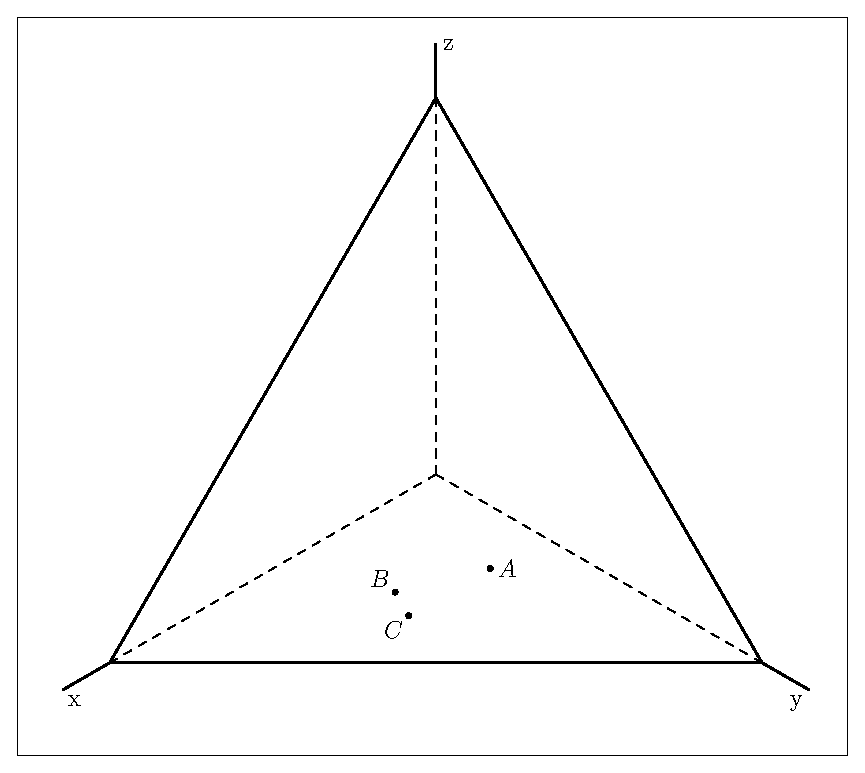
\includegraphics[width=\textwidth]{threepoints.eps}
      \caption{\footnotesize The simplex $\mathbb{S}^{2}$ in
        three-dimensional space $\mathbb{R}^{3}$ with points $a,b,c$
        as in equation (\ref{eq:e6}) representing probability
        distributions $A,B,C$. Note that geometrically speaking $C$ is
        closer to $A$ than $B$ is. Using the Kullback-Leibler
        divergence, however, $B$ is closer to $A$ than $C$ is.}
      \label{fig:threepoints}
    \end{minipage}
  \end{flushright}
\end{figure}

Global inaccuracy reflects the Euclidean proximity relation, not the
re\-commendation of information theory. If $A$ corresponds to my prior
and my evidence is such that I must change the first coordinate to
$1/2$ (as in {\xample}~\ref{ex:holmes}) and nothing stronger, then
information theory via the Kullback-Leibler divergence re\-commends
the posterior corresponding to $B$; and the geometry of reason as
expounded in Leitgeb and Pettigrew recommends the posterior
corresponding to $C$. There are several things going on here that need
some explanation.

\subsection{Evaluating Partial Beliefs in Light of Others}
\label{subsec:aichavag}

We note that for Leitgeb and Pettigrew, expected global inaccuracy of
$b'$ is always evaluated by the lights of another partial belief
distribution $b$. This may sound counterintuitive. Should we not
evaluate $b'$ by its own lights? It is part of a larger Bayesian
commitment that partial belief distributions are not created ex
nihilo. They can also not be evaluated for inaccuracy ex nihilo.
Leitgeb and Pettigrew say very little about this, but it appears that
there is a deeper problem here with the flow of diachronic updating.
The classic Bayesian picture is one of moving from a relatively prior
probability distribution to a posterior distribution (distinguish
relatively prior probability distributions, which precede posterior
probability distributions in updating, from absolutely prior
probability distributions, which are ignorance priors in the sense
that they are not the resulting posteriors of previous updating). This
is nicely captured by standard conditioning, Bayes' formula, and
updating on the basis of information theory (Jeffrey conditioning,
principle of maximum entropy).

The geometry of reason and notions of accuracy based on it sit
uncomfortably with this idea of flow, as the suggestion is that
partial belief distributions are evaluated on their accuracy without
reference to prior probability distributions---why should the
accuracy or epistemic utility of a posterior probability distribution
depend on a prior probability distribution which has already been
debunked by the evidence? I agree with Leitgeb and Pettigrew that
there is no alternative here but to evaluate the posterior by the
lights of the prior. Not doing so would saddle us with Carnap's
Straight Rule, where priors are dismissed as irrelevant (see
\scite{8}{carnap52}{40ff}). Yet we shall note that a justification of
evaluating a belief function's accuracy by the lights of another
belief function is a lot less persuasive than the way Bayesians and
information theory integrate prior distributions into forming
posterior distributions by virtue of an asymmetric flow of
information (see also \scite{7}{shogenji12}{}, who makes a strong case
for the influence of prior probabilities on epistemic justification).

\subsection{LP conditioning and Jeffrey Conditioning}
\label{subsec:meexughi}

I want to outline how Leitgeb and Pettigrew arrive at posterior
probability distributions in Jeffrey-type updating scenarios. I will
call their method LP conditioning.

\begin{quotex}
  \beispiel{Abstract Holmes}\label{ex:abstract} Consider a possibility
  space $W=E_{1}\cup{}E_{2}\cup{}E_{3}$ (the $E_{i}$ are sets of
  states which are pairwise disjoint and whose union is $W$) and a
  partition $\mathcal{F}$ of $W$ such that
  $\mathcal{F}=\{F^{*},F^{**}\}=\{E_{1},E_{2}\cup{}E_{3}\}$.
\end{quotex}

Let $P$ be the prior probability function on $W$ and $P'$ the
posterior. I will keep the notation informal to make this simple, not
mathematically precise. Jeffrey-type updating scenarios give us new
information on the posterior probabilities of partitions such as
$\mathcal{F}$. In {\xample} \ref{ex:abstract}, let

\begin{equation}
  \label{eq:priors}
  \begin{array}{rcl}
    P(E_{1})&=&1/3 \\
    P(E_{2})&=&1/2 \\
    P(E_{3})&=&1/6
  \end{array}
\end{equation}

and the new evidence constrain $P'$ such that
$P'(F^{*})=1/2=P'(F^{**})$.

Jeffrey conditioning works on the following intuition, which elsewhere
I have called Jeffrey's updating principle \textsc{jup} (see also
\scite{7}{wagner02}{}). The posterior probabilities conditional on the
partition elements equal the prior probabilities conditional on the
partition elements since we have no information in the evidence that
they should have changed. Hence,

\begin{align}
  \label{eq:jc}
  &P'_{\mbox{\tiny JC}}(E_{i})&=&P'(E_{i}|F^{*})P'(F^{*})+P'(E_{i}|F^{**})P'(F^{**})\notag \\
  &&=&P(E_{i}|F^{*})P'(F^{*})+P(E_{i}|F^{**})P'(F^{**})
\end{align}

Jeffrey conditioning is controversial (for an introduction to Jeffrey
conditioning see \scite{7}{jeffrey65}{}; for its statistical and
formal properties see \scite{7}{diaconiszabell82}{}; for a pragmatic
vindication of Jeffrey conditioning see \scite{7}{armendt80}{}, and
\scite{7}{skyrms86}{}; for criticism see
\scite{7}{howsonfranklin94}{}). Information theory, however, supports
Jeffrey conditioning. Leitgeb and Pettigrew show that Jeffrey
conditioning does not in general pick out the minimally inaccurate
posterior probability distribution. If the geometry of reason as
presented in Leitgeb and Pettigrew is sound, this would constitute a
powerful criticism of Jeffrey conditioning. Leitgeb and Pettigrew
introduce an alternative to Jeffrey conditioning, which I call LP
conditioning. It proceeds as follows for {\xample} \ref{ex:abstract}
and in general provides the minimally inaccurate posterior probability
distribution in Jeffrey-type updating scenarios.

Solve the following two equations for $x$ and $y$:

\begin{equation}
  \label{eq:lpce}
  \begin{array}{rcl}
    P(E_{1})+x&=&P'(F^{*}) \\
    P(E_{2})+y+P(E_{3})+y&=&P'(F^{**})
  \end{array}
\end{equation}

and then set

\begin{equation}
  \label{eq:lpcf}
  \begin{array}{rcl}
    P'_{\mbox{\tiny LP}}(E_{1})&=&P(E_{1})+x \\
    P'_{\mbox{\tiny LP}}(E_{2})&=&P(E_{2})+y \\
    P'_{\mbox{\tiny LP}}(E_{3})&=&P(E_{3})+y
  \end{array}
\end{equation}

For the more formal and more general account see
\scite{8}{leitgebpettigrew10ii}{254}. The results for {\xample}
\ref{ex:abstract} are:

\begin{equation}
  \label{eq:lpcres}
  \begin{array}{rcl}
    P'_{\mbox{\tiny LP}}(E_{1})&=&1/2 \\
    P'_{\mbox{\tiny LP}}(E_{2})&=&5/12 \\
    P'_{\mbox{\tiny LP}}(E_{3})&=&1/12
  \end{array}
\end{equation}

Compare these results to the results of Jeffrey conditioning:

\begin{equation}
  \label{eq:jcres}
  \begin{array}{rcl}
    P'_{\mbox{\tiny JC}}(E_{1})&=&1/2 \\
    P'_{\mbox{\tiny JC}}(E_{2})&=&3/8 \\
    P'_{\mbox{\tiny JC}}(E_{3})&=&1/8
  \end{array}
\end{equation}

Note that (\ref{eq:priors}), (\ref{eq:jcres}), and (\ref{eq:lpcres})
correspond to $A,B,C$ in (\ref{eq:e6}). 

\subsection{Triangulating LP and Jeffrey Conditioning}
\label{subsec:ieseiwoh}

There is an interesting connection between LP conditioning and Jeffrey
conditioning as updating methods. Let $B$ be on the zero-sum line
between $A$ and $C$ if and only if

\begin{equation}
\label{eq:jooziphu}
d(A,C)=d(A,B)+d(B,C)
\end{equation}

where $d$ is the difference measure we are using, so $d(A,B)=\|B-A\|$
for the geometry of reason and $d(A,B)=D_{\mbox{\tiny KL}}(B,A)$ for
information geometry. For the geometry of reason (and Euclidean
geometry), the zero-sum line between two probability distributions is
just what we intuitively think of as a straight line: in Cartesian
coordinates, $B$ is on the zero-sum line strictly between $A$ and $C$
if and only if for some $\vartheta\in(0,1)$,
$b_{i}=\vartheta{}a_{i}+(1-\vartheta)c_{i}$ and $i=1,\ldots,n$.

What the zero-sum line looks like for information theory is
illustrated in figure \ref{fig:eugoohue}. The reason for the oddity is
that the Kullback-Leibler divergence does not obey
\textsc{triangularity}, an issue that I will address in detail in
subsection \ref{subsec:triangularity}). Call $B$ a zero-sum point
between $A$ and $C$ if (\ref{eq:jooziphu}) holds true. For the
geometry of reason, the zero-sum points are simply the points on the
straight line between $A$ and $C$. For information geometry, the
zero-sum points are the boundary points of the set where you can take a
shortcut by making a detour, i.e.\ all points for which
$d(A,B)+d(B,C)<d(A,C)$.

\begin{figure}[ht]
    \begin{minipage}[h]{.7\linewidth}
      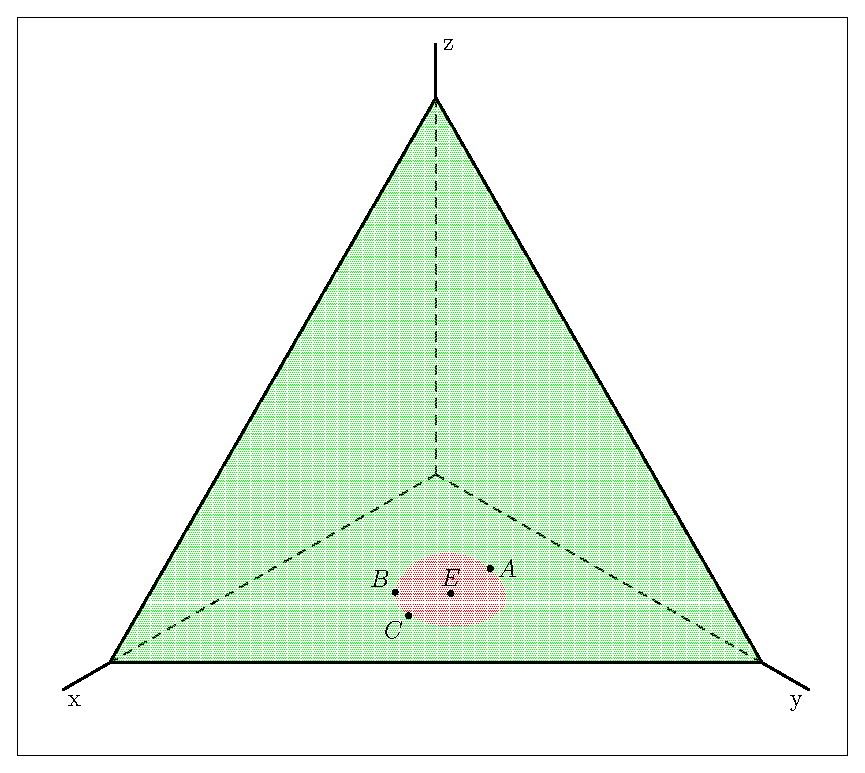
\includegraphics[width=\textwidth]{dreieck.eps}
      \caption{The zero-sum line between $A$ and $C$ is the boundary
        line between the green area, where the triangle inequality
        holds, and the red area, where the triangle inequality is
        violated. The posterior probability distribution $B$
        recommended by Jeffrey conditioning always lies on the
        zero-sum line between the prior $A$ and the LP posterior $C$,
        as per equation (\ref{eq:ocidocho}). $E$ is the point in the
        red area where the triangle inequality is most efficiently
        violated.}
      \label{fig:eugoohue}
\end{minipage}
\end{figure}

Remarkably, if $A$ represents a relatively prior probability
distribution and $C$ the posterior probability distribution
recommended by LP conditioning, the posterior probability distribution
recommended by Jeffrey conditioning is always a zero-sum point with
respect to the Kullback-Leibler divergence:

\begin{equation}
  \label{eq:ocidocho}
  D_{\mbox{\tiny KL}}(C,A)=D_{\mbox{\tiny KL}}(B,A)+D_{\mbox{\tiny KL}}(C,B)
\end{equation}

Informationally speaking, if you go from $A$ to $C$, you can just as
well go from $A$ to $B$ and then from $B$ to $C$. This does not mean
that we can conceive of information geometry the way we would conceive
of non-Euclidean geometry, where it is also possible to travel faster
on what from a Euclidean perspective looks like a detour. For in
information geometry, you can travel faster on what from the
perspective of information theory (!) looks like a detour, i.e.\ the
triangle inequality does not hold. 

To prove equation (\ref{eq:ocidocho}) in the case $n=3$ (assuming that
LP conditioning does not \qnull{fall off the edge} as in case (b) in
\scite{8}{leitgebpettigrew10ii}{253}) note that all three points
(prior, point recommended by Jeffrey conditioning, point recommended
by LP conditioning) can be expressed using three variables:

\begin{equation}
  \label{eq:reejeiru}
  \begin{array}{rcl}
    A&=&\left(1-\alpha,\beta,\alpha-\beta\right) \\
     && \\
    B&=&\left(1-\gamma,\frac{\gamma\beta}{\alpha},\frac{\gamma(\alpha-\beta)}{\alpha}\right) \\
     && \\
    C&=&\left(1-\gamma,\beta+\frac{1}{2}(\gamma-\alpha),\alpha-\beta+\frac{1}{2}(\gamma-\alpha)\right)
  \end{array}
\end{equation}

The rest is basic algebra using the definition of the Kullback-Leibler
divergence in (\ref{eq:e7}). To prove the claim for arbitrary $n$
one simply generalizes (\ref{eq:reejeiru}). It is a handy corollary of
(\ref{eq:ocidocho}) that whenever $(A,B)$ and $(B,C)$ violate
\textsc{transitivity of asymmetry} then 

\begin{equation}
  \label{eq:saithain}
  D_{\mbox{\tiny KL}}(A,C)>D_{\mbox{\tiny KL}}(B,C)+D_{\mbox{\tiny KL}}(A,B)
\end{equation}

in violation of \textsc{triangularity}. This way I will not have to
go hunting for an example to demonstrate the violation of
\textsc{triangularity}. $A,B,C$ of (\ref{eq:e6}) fulfill all the
conditions for (\ref{eq:saithain}) and therefore violate
\textsc{triangularity}.

It is an interesting question to wonder which point $E$ violates the
triangle inequality most efficiently so that

\begin{equation}
  \label{eq:eaghaidu}
D_{\mbox{\tiny KL}}(E,C)+D_{\mbox{\tiny KL}}(A,E)  
\end{equation}

is minimal. Let $e=(e_{1},\ldots,e_{n})$ represent $E$ in
$\mathbb{S}^{n-1}$. Use the Lagrange Multiplier method to find the
Lagrangian

\begin{equation}
  \label{eq:eiweehee}
  \mathcal{L}(e,\lambda)=\sum_{i=1}^{n}e_{i}\log\frac{e_{i}}{a_{i}}+\sum_{i=1}^{n}c_{i}\log\frac{c_{i}}{e_{i}}+\lambda\left(\sum_{i=1}^{n}e_{i}-1\right)
\end{equation}

The Lagrange Multiplier method gives us

\begin{equation}
  \label{eq:nainguji}
  \frac{\partial\mathcal{L}}{\partial{}e_{k}}=\log\frac{e_{k}}{a_{k}}+1-\frac{r}{q}+\lambda=0\mbox{ for each }k=1,{\ldots},n.
\end{equation}

Manipulate this equation to yield

\begin{equation}
  \label{eq:ohjoogoh}
  \frac{c_{k}}{e_{k}}\exp\left(\frac{c_{k}}{e_{k}}\right)=\frac{c_{k}}{a_{k}}\exp(1+\lambda).
\end{equation}

To solve (\ref{eq:ohjoogoh}), use the Lambert W function

\begin{equation}
  \label{eq:ouquuzoh}
  e_{k}=\frac{c_{k}}{W\left(\frac{c_{k}}{a_{k}}\exp(1+\lambda)\right)}.
\end{equation}

Choose $\lambda$ to fulfill the constraint $\sum{}e_{i}=1$. The
result for the discrete case accords with Ovidiu Calin and Constantin
Udriste's result for the continuous case (see equation 4.7.9 in
\scite{8}{calinudriste14}{127}). Numerically, for $A$ and $C$ as
defined in equation (\ref{eq:e6}),

\begin{equation}
  \label{eq:aemaujei}
  E=(0.415,0.462,0.123).
\end{equation}

This is subtly different from the midpoint $m_{i}=0.5a_{i}+0.5c_{i}$
(if we were minimizing
$D_{\mbox{\tiny KL}}(A,E)+D_{\mbox{\tiny KL}}(C,E)$, the solution
would be the midpoint). I do not know whether $A,E,C$ are collinear
(see figure \ref{fig:eugoohue} for illustration).

\section{Expectations for the Geometry of Reason}
\label{fivex}

This section provides more detail for the expectations in \textbf{List
  A} and shows how LP conditioning violates them.

\subsection{Continuity}
\label{Continuity}

LP conditioning violates \textsc{continuity} because standard
conditioning gives a different recommendation than a parallel sequence
of Jeffrey-type updating scenarios which get arbitrarily close to
standard event observation. This is especially troubling considering
how important the case for standard conditioning is to Leitgeb and
Pettigrew.

To illustrate a \textsc{continuity} violation, consider the case where
Sherlock Holmes reduces his credence that the culprit was male to
$\varepsilon_{n}=1/n$ for $n=4,5,\ldots$. The sequence
$\varepsilon_{n}$ is not meant to reflect a case where Sherlock Holmes
becomes successively more certain that the culprit was female. It is
meant to reflect countably many parallel scenarios which only differ
by the degree to which Sherlock Holmes is sure that the culprit was
female. These parallel scenarios give rise to a parallel sequence (as
opposed to a successive sequence) of updated probabilities
$P'_{\mbox{\tiny LP}}(F^{**})$ and another sequence of updated
probabilities $P'_{\mbox{\tiny JC}}(F^{**})$ ($F^{**}$ is the
proposition that the culprit is female). As $n\rightarrow\infty$, both
of these sequences go to one.

Straightforward conditionalization on the evidence that \qnull{the
  culprit is female} gives us 

\begin{equation}
  \label{eq:sherlockcontsc}
  \begin{array}{rcl}
  P'_{\mbox{\tiny SC}}(E_{1})&=&0\\
  P'_{\mbox{\tiny SC}}(E_{2})&=&3/4\\
  P'_{\mbox{\tiny SC}}(E_{3})&=&1/4.
\end{array}
\end{equation}

Letting $n\rightarrow\infty$ for Jeffrey conditioning yields

\begin{equation}
  \label{eq:sherlockcontjc}
  \begin{array}{rcccl}
  P'_{\mbox{\tiny JC}}(E_{1})&=&1/n&\rightarrow&0\\
  P'_{\mbox{\tiny JC}}(E_{2})&=&3(n-1)/4n&\rightarrow&3/4\\
  P'_{\mbox{\tiny JC}}(E_{3})&=&(n-1)/4n&\rightarrow&1/4,
\end{array}
\end{equation}

whereas letting $n\rightarrow\infty$ for LP conditioning yields

\begin{equation}
  \label{eq:sherlockcontlp}
  \begin{array}{rcccl}
  P'_{\mbox{\tiny LP}}(E_{1})&=&1/n&\rightarrow&0\\
  % this is mine, further down is Paul's 
  % P'_{\mbox{\tiny LP}}(E_{2})&=&(4n-1)/6n&\rightarrow&2/3\\
  % P'_{\mbox{\tiny LP}}(E_{3})&=&(2n-1)/6n&\rightarrow&1/3.
  P'_{\mbox{\tiny LP}}(E_{2})&=&(4n-3)/6n&\rightarrow&2/3\\
  P'_{\mbox{\tiny LP}}(E_{3})&=&(2n-5)/6n&\rightarrow&1/3.
\end{array}
\end{equation}

LP conditioning violates \textsc{continuity}.

\subsection{Regularity}
\label{Regularity}

LP conditioning violates \textsc{regularity} because formerly positive
probabilities can be reduced to $0$ even though the new information in
the Jeffrey-type updating scenario makes no such requirements (as is
usually the case for standard conditioning). Ironically, Jeffrey-type
updating scenarios are meant to be a better reflection of real-life
updating because they avoid extreme probabilities. 

The violation becomes serious if we are already sympathetic to an
infor\-ma\-tion-based account: the amount of information required to turn
a non-extreme probability into one that is extreme ($0$ or $1$) is
infinite. Whereas the geometry of reason considers extreme
probabilities to be easily accessible by non-extreme probabilities
under new information (much like a marble rolling off a table or a
bowling ball heading for the gutter), information theory envisions
extreme probabilities more like an event horizon. The nearer you are
to the extreme probabilities, the more information you need to move
on. For an observer, the horizon is never reached.

\begin{quotex}
  \beispiel{Regularity Holmes}\label{ex:regularity} Everything is as
  in {\xample} \ref{ex:holmes}, except that Sherlock Holmes becomes
  confident to a degree of $2/3$ that Mr.\ R is the culprit and
  updates his relatively prior probability distribution in
  (\ref{eq:priors}).
\end{quotex}

Then his posterior probabilities look as follows:

\begin{equation}
  \label{eq:sherlockposteriorjcreg}
  \begin{array}{rcl}
  P'_{\mbox{\tiny JC}}(E_{1})&=&2/3\\
  P'_{\mbox{\tiny JC}}(E_{2})&=&1/4\\
  P'_{\mbox{\tiny JC}}(E_{3})&=&1/12
\end{array}
\end{equation}

\begin{equation}
  \label{eq:sherlockposteriorlpreg}
  \begin{array}{rcl}
  P'_{\mbox{\tiny LP}}(E_{1})&=&2/3\\
  P'_{\mbox{\tiny LP}}(E_{2})&=&1/3\\
  P'_{\mbox{\tiny LP}}(E_{3})&=&0
\end{array}
\end{equation}

With LP conditioning, Sherlock Holmes' subjective probability that
Ms.\ T is the culprit in {\xample} \ref{ex:regularity} has been reduced
to zero. No finite amount of information could bring Ms.\ T back into
consideration as a culprit in this crime, and Sherlock Holmes should
be willing to bet any amount of money against a penny that she is not
the culprit---even though his evidence is nothing more than an
increase in the probability that Mr.\ R is the culprit.

LP conditioning violates \textsc{regularity}.

\subsection{Levinstein}
\label{Levinstein}

LP conditioning violates \textsc{levinstein} because of \qeins{the
  potentially dramatic effect [LP conditioning] can have on the
  likelihood ratios between different propositions}
\scite{3}{levinstein12}{419}. Consider Benjamin Levinstein's example:

\begin{quotex}
  \beispiel{Levinstein's Ghost}\label{ex:levinstein} There is a car
  behind an opaque door, which you are almost sure is blue but which
  you know might be red. You are almost certain of materialism, but
  you admit that there's some minute possibility that ghosts exist.
  Now the opaque door is opened, and the lighting is fairly good. You
  are quite surprised at your sensory input: your new credence that
  the car is red is very high.
\end{quotex}

Jeffrey conditioning leads to no change in opinion about ghosts. Under
LP conditioning, however, seeing the car raises the probability that
there are ghosts to an astonishing 47\%, given Levinstein's reasonable
priors. Levinstein proposes a logarithmic inaccuracy measure as a
remedy to avoid violation of \textsc{levinstein}. As a special case of
applying a Levinstein-type logarithmic inaccuracy measure, information
theory does not violate \textsc{levinstein}.

\subsection{Invariance}
\label{Invariance}

LP conditioning violates \textsc{invariance} because two agents who
have identical credences with respect to a partition of the event
space may disagree about this partition after LP conditioning, even
when the Jeffrey-type updating scenario provides no new information
about the more finely grained partitions on which the two agents
disagree. 

\begin{quotex}
  \beispiel{Jane Marple}\label{ex:marple} Jane Marple is on the same
  case as Sherlock Holmes in {\xample} \ref{ex:holmes} and arrives at
  the same relatively prior probability distribution as Sherlock
  Holmes (I will call Jane Marple's relatively prior probability
  distribution $Q$ and her posterior probability distribution $Q'$).
  Jane Marple, however, has a more finely grained probability
  assignment than Sherlock Holmes and distinguishes between the case
  where Ms.\ S went to boarding school with her, of which she has a
  vague memory, and the case where Ms.\ S did not and the vague memory
  is only about a fleeting resemblance of Ms.\ S with another boarding
  school mate. Whether or not Ms.\ S went to boarding school with Jane
  Marple is completely beside the point with respect to the crime, and
  Jane Marple considers the possibilities equiprobable whether or not
  Ms.\ S went to boarding school with her.
\end{quotex}

Let $E_{2}\equiv{}E_{2}^{*}\vee{}E_{2}^{**}$, where $E_{2}^{*}$ is the
proposition that Ms.\ S is the culprit and she went to boarding school
with Jane Marple and $E_{2}^{**}$ is the proposition that Ms.\ S is
the culprit and she did not go to boarding school with Jane Marple.
Then

\begin{equation}
  \label{eq:marpleprior}
  \begin{array}{rcl}
  Q(E_{1})&=&1/3\\
  Q(E_{2}^{*})&=&1/4\\
  Q(E_{2}^{**})&=&1/4\\
  Q(E_{3})&=&1/6.
\end{array}
\end{equation}

Now note that while Sherlock Holmes and Jane Marple agree on the
relevant facts of the criminal case (who is the culprit?) in their
posterior probabilities if they use Jeffrey conditioning,

\begin{equation}
  \label{eq:sherlockposteriorjc}
  \begin{array}{rcl}
  P'_{\mbox{\tiny JC}}(E_{1})&=&1/2\\
  P'_{\mbox{\tiny JC}}(E_{2})&=&3/8\\
  P'_{\mbox{\tiny JC}}(E_{3})&=&1/8
\end{array}
\end{equation}

\begin{equation}
  \label{eq:marpleposteriorjc}
  \begin{array}{rcl}
  Q'_{\mbox{\tiny JC}}(E_{1})&=&1/2\\
  Q'_{\mbox{\tiny JC}}(E_{2}^{*})&=&3/16\\
  Q'_{\mbox{\tiny JC}}(E_{2}^{**})&=&3/16\\
  Q'_{\mbox{\tiny JC}}(E_{3})&=&1/8
\end{array}
\end{equation}

they do not agree if they use LP conditioning,

\begin{equation}
  \label{eq:sherlockposteriorlp}
  \begin{array}{rcl}
  P'_{\mbox{\tiny LP}}(E_{1})&=&1/2\\
  P'_{\mbox{\tiny LP}}(E_{2})&=&5/12\\
  P'_{\mbox{\tiny LP}}(E_{3})&=&1/12
\end{array}
\end{equation}

\begin{equation}
  \label{eq:marpleposteriorlp}
  \begin{array}{rcl}
  Q'_{\mbox{\tiny LP}}(E_{1})&=&1/2\\
  Q'_{\mbox{\tiny LP}}(E_{2}^{*})&=&7/36\\
  Q'_{\mbox{\tiny LP}}(E_{2}^{**})&=&7/36\\
  Q'_{\mbox{\tiny LP}}(E_{3})&=&1/9.
\end{array}
\end{equation}

LP conditioning violates \textsc{invariance}.

\subsection{Expansibility}
\label{Expansibility}

One particular problem with the lack of invariance for LP conditioning
is how zero-probability events should be included in the list of prior
probabilities that determines the value of the posterior
probabilities. Consider

\begin{equation}
  \label{eq:reginvone}
  \begin{array}{rcl}
  P(X_{1})&=&0\\
  P(X_{2})&=&0.3\\
  P(X_{3})&=&0.6\\
  P(X_{4})&=&0.1\\
\end{array}
\end{equation}

That $P(X_{1})=0$ may be a consequence of standard conditioning in a
previous step. Now the agent learns that $P'(X_{3}\vee{}X_{4})=0.5$.
Should the agent update on the list presented in (\ref{eq:reginvone})
or on the following list:

\begin{equation}
  \label{eq:reginvtwo}
  \begin{array}{rcl}
  P(X_{2})&=&0.3\\
  P(X_{3})&=&0.6\\
  P(X_{4})&=&0.1\\
\end{array}
\end{equation}

Whether you update on (\ref{eq:reginvone}) or (\ref{eq:reginvtwo})
makes no difference to Jeffrey conditioning, but due to the lack of
invariance it makes a difference to LP conditioning, so the geometry
of reason needs to find a principled way to specify the appropriate
prior probabilities. The only non-arbitrary way to do this is either
to include or to exclude all zero probability events on the list. This
strategy, however, sounds ill-advised unless one signs on to a
stronger version of \textsc{regularity} and requires that only a fixed
set of events can have zero probabilities (such as logical
contradictions), but then the geometry of reason ends up in the
catch-22 of LP conditioning running afoul of \textsc{regularity}.

LP conditioning violates \textsc{expansibility}.

\subsection{Horizon}
\label{Horizon}

\begin{quotex}
  \beispiel{Undergraduate Complaint}\label{ex:complaint} An
  undergraduate student complains to the department head that the
  professor will not reconsider an 89\% grade (which misses an A+ by
  one percent) when reconsideration was given to other students with a
  67\% grade (which misses a B- by one percent).
\end{quotex}

Intuitions may diverge, but the professor's reasoning is as follows.
To improve a 60\% paper by ten percent is easily accomplished: having
your roommate check your grammar, your spelling, and your line of
argument will sometimes do the trick. It is incomparably more
difficult to improve an 85\% paper by ten percent: it may take doing a
PhD to turn a student who writes the former into a student who writes
the latter. A maiore ad minus, the step from 89\% to 90\% is greater
than the step from 67\% to 68\%.

Another example for the horizon effect is George Schlesinger's
comparison between the risk of a commercial airplane crash and the
risk of a military glider landing in enemy territory.

\begin{quotex}
  \beispiel{Airplane Gliders}\label{ex:schlesinger} Compare two
  scenarios. In the first, an airplane which is considered safe
  (probability of crashing is $1/10^{9}$) goes through an
  inspection where a mechanical problem is found which increases
  the probability of a crash to $1/100$. In the second, military
  gliders land behind enemy lines, where their risk of perishing
  is 26\%. A slight change in weather pattern increases this risk
  to 27\%. \scite{3}{schlesinger95}{211}
\end{quotex}

For an interesting instance of the horizon effect in asymmetric
multi-dimen\-sional scaling see \scite{7}{chinoshiraiwa93}{}, section 3,
where Naohito Chino and Kenichi Shiraiwa describe as one of the
properties of their Hilbert space models of asymmetry how \qeins{the
  similarity between the pair of objects located far from the centroid
  of objects, say, the origin, is greater than that located near the
  origin, even if their distances are the same} (42).

I claim that an amujus ought to fulfill the requirements of the
horizon effect: it ought to be more difficult to update as
probabilities become more extreme (or less middling). I have
formalized this requirement in \textbf{List B}. It is trivial that the
geometry of reason does not fulfill it. Information theory fails as
well, which gives the horizon effect its prominent place in both
lists. The way information theory fails, however, is quite different.
Near the boundary of $\mathbb{S}^{n-1}$, information theory reflects
the horizon effect just as our expectation requires. The problem is
near the centre, where some equidistant points are more divergent the
closer they are to the middle. I will give an example and more
explanation in subsection \ref{subsec:colhor}.

In the next section, I will closely tie the issue of the horizon
effect to confirmation. The two main candidates for quantitative
measures of relevance confirmation disagree on precisely this issue.
Whether you, the reader, will accept the horizon requirement may
depend on what your view is on degree of confirmation theory.

\subsection{Confirmation}
\label{Confirmation}

The geometry of reason thinks about the comparison of probability
distributions in terms of distance. Information theory thinks about
the comparison along the lines of information loss when one
distribution is used to encode a message rather than the other
distribution. One way to test these approaches is to ask how well they
align with a third approach to such a comparison: degree of
confirmation. Our main concern is the horizon effect of the previous
subsection. Which approaches to degree of confirmation theory reflect
it, and how do these approaches correspond to the disagreements
between information theory and the geometry of reason?

There is, of course, a relevant difference between the aims of the
epistemic utility approach to updating and the aims of degree of
confirmation theory. The former investigates norms to which a rational
agent conforms in her pursuit of epistemic utility. The latter seeks to
establish qualitative and quantitative measures of impact that
evidence has on a hypothesis. Both, however, (I will restrict my
attention here to quantitative degree of confirmation theory) attend
to the probability of an event, which degree of confirmation theory
customarily calls $h$ for hypothesis, before and after the rational
agent processes another event, customarily called $e$ for evidence,
i.e.\ $x=P(h|k)$ and $y=P(h|e,k)$ ($k$ is background information).

For perspectives on the link between confirmation and information see
\scite{8}{shogenji12}{37f}; \scite{7}{crupitentori14}{}; and
\scite{7}{milne14}{}, section 4. Vincenzo Crupi and Katya Tentori
suggest that there is a \qeins{parallelism between confirmation and
  information search [which] can serve as a valuable heuristic for
  theoretical work} \scite{3}{crupitentori14}{89}. 

In degree of confirmation theory, incremental confirmation is
distinguished from absolute confirmation in the following sense. Let
$h$ be the presence of a very rare disease and $e$ a test result such
that $y>>x$ but $y<1-y$. Then, absolutely speaking, $e$ disconfirms
$h$ (for Rudolf Carnap, absolute confirmation involves sending $y$
above a threshold $r$ which must be greater than or equal to $0.5$).
Absolute confirmation is not the subject of this section. I will
exclusively discuss incremental confirmation (also called relevance
confirmation, just as absolute confirmation is sometimes called
firmness confirmation) where $y>x$ implies (incremental) confirmation,
$y<x$ implies (incremental) disconfirmation, and $y=x$ implies the
lack of both. The difference is illustrated in figure
\ref{fig:doconf}.

All proposed measures of quantitative, incremental degree of
confirmation considered here are a function of $x$ and $y$. Dependence
of incremental confirmation on only $x$ and $y$ is not trivial, as
$P(e|k)$ and $P(e|h,k)$ cannot be expressed using only $x$ and $y$
(for a case why dependence should be on only $x$ and $y$ see
\scite{8}{atkinson12}{50}, with an irrelevant conjunction argument;
and \scite{8}{milne14}{254}, with a continuity argument). David
Christensen's measure $P(h|e,k)-P(h|\urcorner{}e,k)$ (see
\scite{8}{christensen99}{449}) and Robert Nozick's
$P(e|h,k)-P(e|\urcorner{}h,k)$ (see \scite{8}{nozick81}{252}) are not
only dependent on $x$ and $y$, but also on $P(e|k)$, which makes them
vulnerable to Atkinson's and Milne's worries just cited.

Consider the following six contenders for a quantitative, incremental
degree of confirmation function, dependent on only $x$ and $y$. They
are based on, in a brief slogan, (i) difference of conditional
probabilities, (ii) ratio of conditional probabilities, (iii)
difference of odds, (iv) ratio of likelihoods, (v) Gaifman's treatment
of Hempel's raven paradox, and (vi) conservation of contrapositivity
and commutativity. Logarithms throughout this paper are assumed to be
the natural logarithm in order to facilitate easy differentiation,
although generally a particular choice of base (greater than one) does
not make a relevant difference.

% zahThe2a
\begin{equation}
  \label{eq:relevance}
  \begin{array}{lrcl}
    \mbox{(i) } & M_{P}(x,y)&=&y-x \\
                &&& \\
    \mbox{(ii) } & R_{P}(x,y)&=&\displaystyle\log\frac{y}{x} \\
                &&& \\
    \mbox{(iii) } & J_{P}(x,y)&=&\displaystyle\frac{y}{1-y}-\frac{x}{1-x} \\
                &&& \\
    \mbox{(iv) } & L_{P}(x,y)&=&\displaystyle\log\frac{y(1-x)}{x(1-y)} \\
                &&& \\
    \mbox{(v) } & G_{P}(x,y)&=&\displaystyle\log\frac{1-x}{1-y} \\
                &&& \\
    \mbox{(vi) } & Z_{P}(x,y)&=&\left\{
                                 \begin{array}{cl}
                                   \displaystyle\frac{y-x}{1-x}&\mbox{if }y\geq{}x \\
                                   \displaystyle\frac{y-x}{x}&\mbox{if }y<x
                                 \end{array}\right.
  \end{array}
\end{equation}

$M_{P}$ is defended by \scite{7}{carnap62}{}; \scite{7}{earman92}{};
\scite{7}{rosenkrantz94}{}. $R_{P}$ is defended by
\scite{7}{keynes21}{}; \scite{7}{milne96}{}; \scite{7}{shogenji12}{}.
$J_{P}$ is defended by \scite{7}{festa99}{}. $L_{P}$ is defended by
\scite{7}{good50}{}; \scite{7}{good83}{}, chapter 14;
\scite{7}{fitelson06}{}; \scite{7}{zalabardo09}{}. $G_{P}$ is defended
by \scite{8}{gaifman79}{120}, without the logarithm (I added it to
make $G_{P}$ more comparable to the other functions). $Z_{P}$ is
defended by \scite{7}{crupietal07}{}. For more literature supporting
the various measures consult footnote 1 in
\scite{8}{fitelson01}{S124}; and an older survey of options in
\scite{7}{kyburg83}{}.

To compare how these degree of confirmation measures align with the
concept of difference between probability distributions for the
purpose of updating it is best to look at derivatives as they reflect
the rate of change from the middle to the extremes. This is how we
capture the horizon effect requirement for two dimensions. One
important difference between degree of confirmation theory and
updating is that the former is concerned with a hypothesis and its
negation whereas the latter considers all sorts of domains for the
probability distribution (in this paper, I have restricted myself to a
finite outcome space). As far as the analogy between degree of
confirmation theory on the one hand and updating on the other hand is
concerned, I only need to look at the two-dimensional case.

To discriminate between candidates (i)--(vi), I am setting up three
criteria (complementing many others in the literature). Let $D(x,y)$
be the generic expression for the degree of confirmation function.
Call this \textbf{List C}.

\begin{itemize}
\item \textsc{additivity} A theory can be confirmed piecemeal. Whether
  the evidence is split up into two or more components or left in one
  piece is irrelevant to the amount of confirmation it confers.
  Formally, $D(x,z)=D(x,y)+D(y,z)$. Note that this is not the usual
  triangle inequality because I am in two dimensions.
\item \textsc{skew-antisymmetry} It does not matter whether $h$ or
  $\urcorner{}h$ is in view. Confirmation and disconfirmation are
  commensurable. Formally, $D(x,y)=-D(1-x,1-y)$. A surprising number
  of candidates fail this requirement, and the requirement is not
  common in the literature (see, however, the second clause in Milne's
  fourth desideratum in \scite{10}{milne96}{21}). In defence of this
  requirement consider {\xample} \ref{ex:ieyohjah} below.
  $d_{1}>{}d_{2}$ may have a negative impact on the latter scientist's
  grant application, even though the inequality may solely be due to a
  failure to fulfill skew-antisymmetry.
\item \textsc{confirmation horizon} An account of degree of
  confirmation must exhibit the horizon effect as in \textbf{List A}
  and \textbf{List B}, except more simply in two dimensions. Formally,
  the functions $\partial{}D_{\varepsilon}^{+}/\partial{}x$ must be
  strictly positive and the functions
  $\partial{}D_{\varepsilon}^{-}/\partial{}x$ must be strictly
  negative for all $\varepsilon\in{}(-1/2,1/2)$. These functions are
  defined in (\ref{eq:defdhpos}) and (\ref{eq:defdhneg}), and I prove
  in appendix~\ref{app:horform} that the requirement to keep them
  strictly positive/neg\-ative is equivalent to the horizon effect as
  described formally in \textbf{List B}.
\end{itemize}

\begin{quotex}
  \beispiel{Grant Adjudication I}\label{ex:ieyohjah} Two scientists
  compete for grant money. Professor X presents an experiment
  conferring degree of confirmation $d_{1}$ on a hypothesis, if
  successful; Professor Y presents an experiment conferring degree of
  disconfirmation $-d_{2}$ on the negation of the same hypothesis, if
  unsuccessful. (For the relevance of quantitative confirmation
  measures to the evaluation of scientific projects see
  \scite{8}{salmon75}{11}.)
\end{quotex}

The functions for the horizon effect are defined as follows. Let
$\varepsilon\in{}(-1/2,1/2)$ be fixed. Recall that $D(x,y)$ is the
generic expression for a confirmation function measuring the degree of
confirmation that a posterior $y=P(h|e,k)$ bestows on a hypothesis for
which the prior is $x=P(h|k)$. $\varepsilon$ is the difference $y-x$.
For $\varepsilon>0$,

\begin{equation}
  \begin{array}{lrcl}
  D_{\varepsilon}^{-}:(0,\frac{1}{2}-\varepsilon)\rightarrow{}\mathbb{R} & D_{\varepsilon}^{-}(x)&=&|D(x,x+\varepsilon)| \\
  D_{\varepsilon}^{+}:(\frac{1}{2},1-\varepsilon)\rightarrow{}\mathbb{R} & D_{\varepsilon}^{+}(x)&=&|D(x,x+\varepsilon)| \\
  \end{array}
  \label{eq:defdhpos}
\end{equation}

For $\varepsilon<0$,

\begin{equation}
  \begin{array}{lrcl}
  D_{\varepsilon}^{-}:(-\varepsilon,\frac{1}{2})\rightarrow{}\mathbb{R} & D_{\varepsilon}^{-}(x)&=&|D(x,x+\varepsilon)| \\
  D_{\varepsilon}^{+}:(\frac{1}{2}-\varepsilon,1)\rightarrow{}\mathbb{R} & D_{\varepsilon}^{+}(x)&=&|D(x,x+\varepsilon)| \\
  \end{array}
  \label{eq:defdhneg}
\end{equation}

The rate of change for the different quantitative measures of degree
of confirmation can be observed in figure \ref{fig:doconf}. The pass
and fail verdicts in the table below are evident from figure
\ref{fig:doconf} and the table of derivatives provided in appendix
\ref{app:horform}. Only $J_{P},L_{P}$ and $Z_{P}$ fulfill the horizon
requirement.

\begin{figure}[ht]
    \begin{minipage}[h]{\linewidth}
      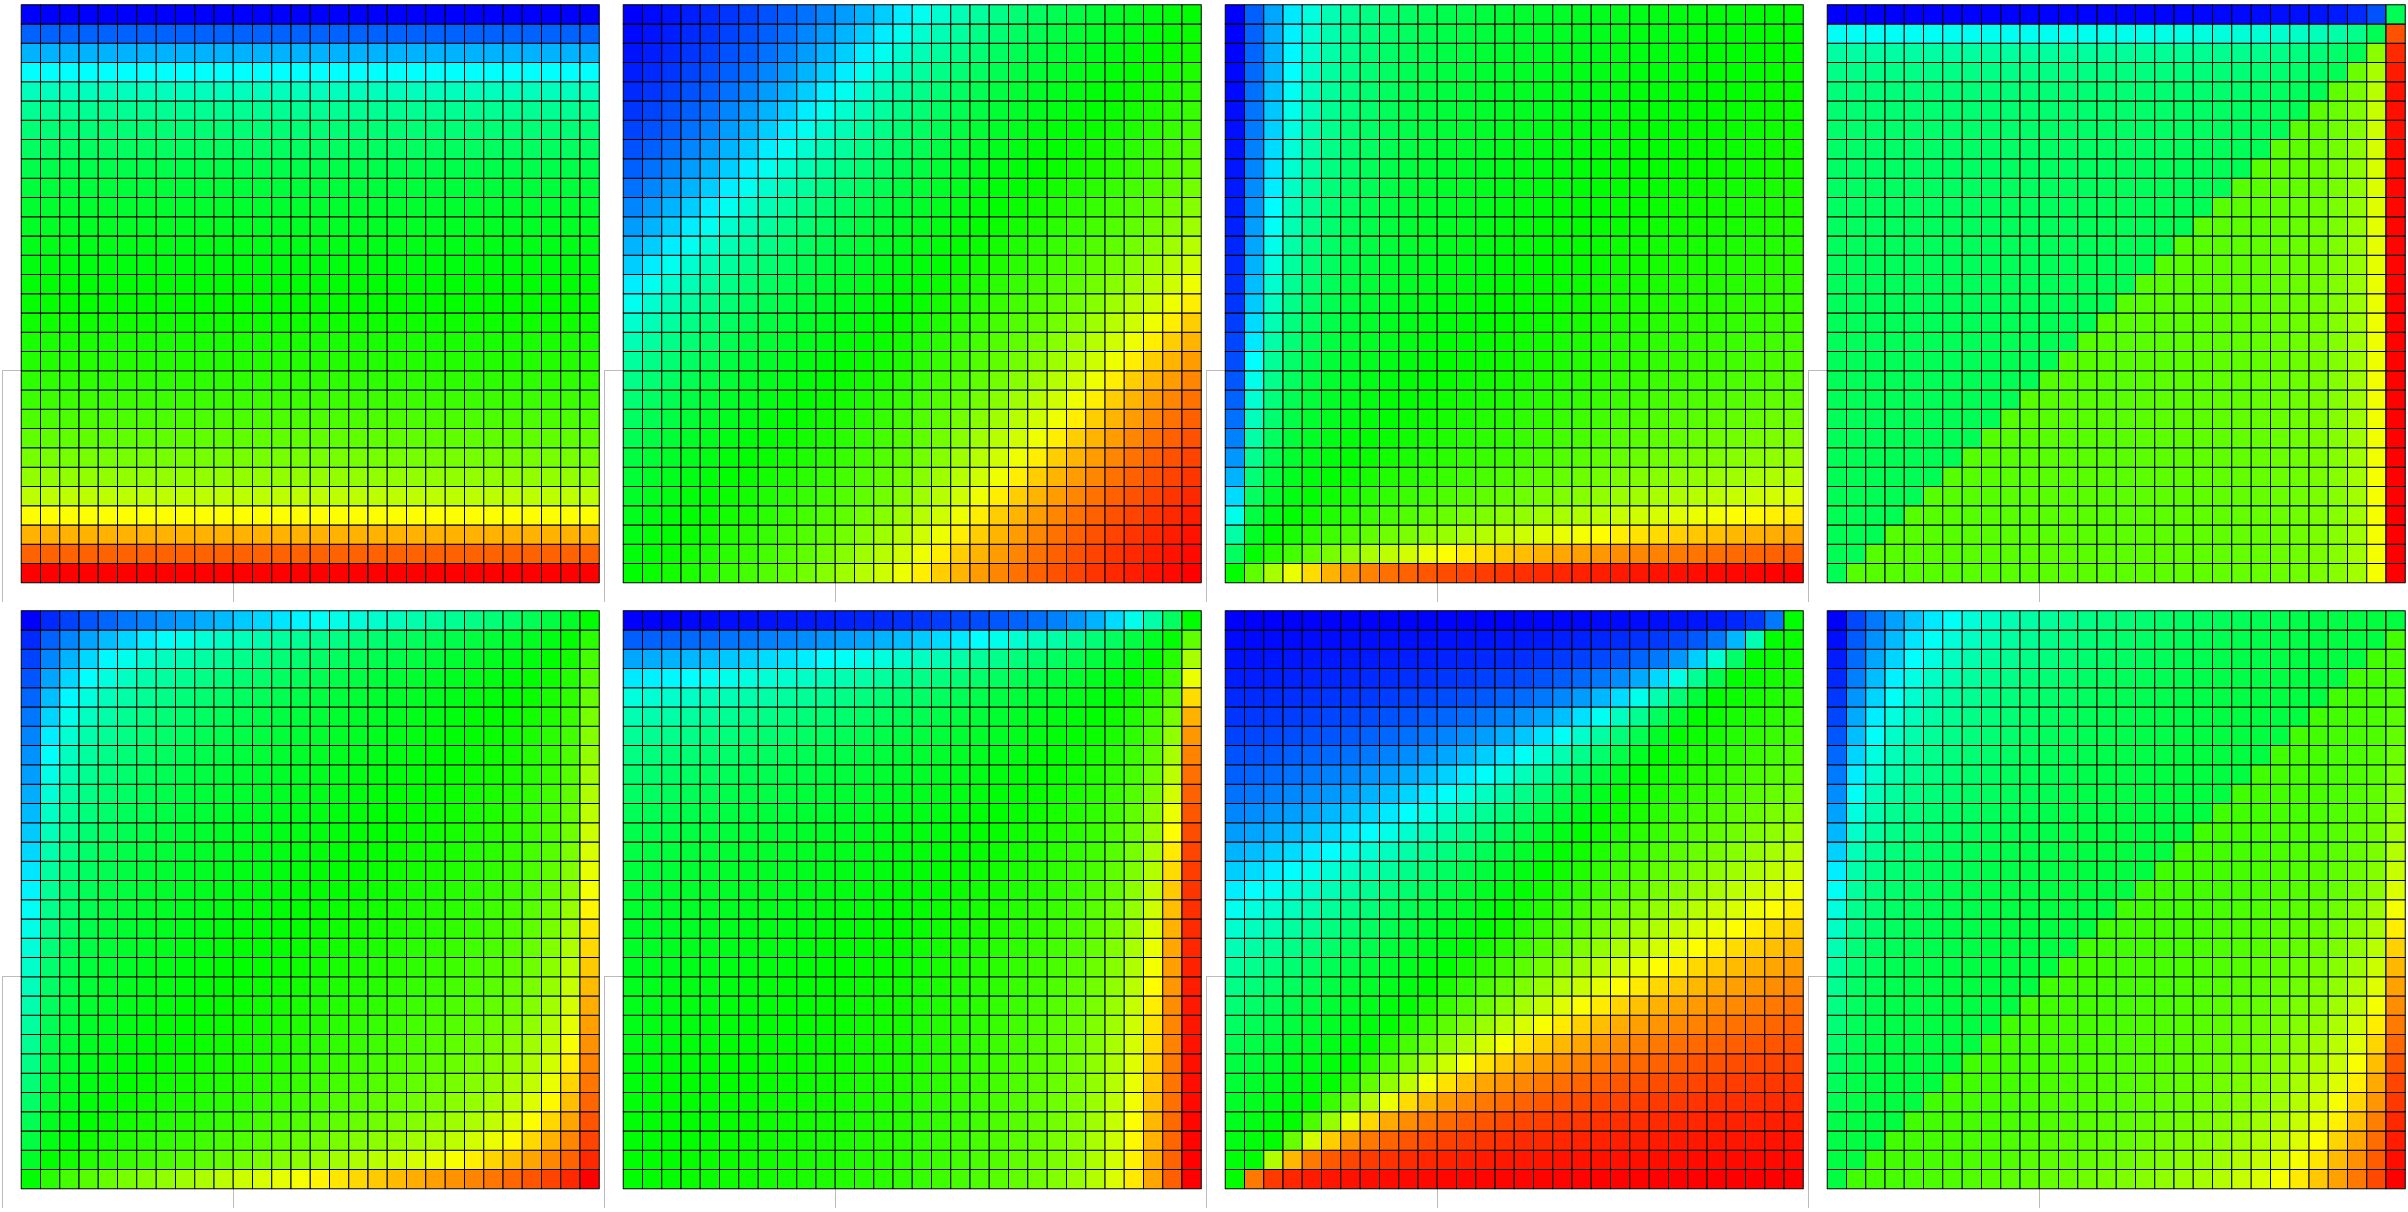
\includegraphics[width=\textwidth]{confirmation-FMRJLGZI.png}
      \caption{\footnotesize Illustration for the six degree of
        confirmation candidates plus Carnap's firmness confirmation
        and the Kullback-Leibler divergence. The top row, from left to
        right, illustrates FMRJ, the bottom row LGZI. \qnull{F} stands
        for Carnap's firmness confirmation measure
        $F_{P}(x,y)=\log(y/(1-y))$. \qnull{M} stands for candidate
        (i), $M_{P}(x,y)$ in (\ref{eq:relevance}), the other letters
        correspond to the other candidates (ii)-(v). \qnull{I} stands
        for the Kullback-Leibler divergence multiplied by the sign
        function of $y-x$ to mimic a quantitative measure of
        confirmation. For all the squares, the colour reflects the
        degree of confirmation with $x$ on the $x$-axis and $y$ on the
        $y$-axis, all between $0$ and $1$. The origin of the square's
        coordinate system is in the bottom left corner. Blue signifies
        strong confirmation, red signifies strong disconfirmation, and
        green signifies the scale between them. Perfect green is
        $x=y$. $G_{P}$ looks like it might pass the horizon
        requirement, but the derivative reveals that it fails
        \textsc{confirmation horizon} (see appendix
        \ref{app:horform}).}
      \label{fig:doconf}
\end{minipage}
\end{figure}

\begin{tabular}{|l|l|l|l|}\hline
  \emph{Candidate} & \emph{Triangularity} & \emph{Skew-Antisymmetry} & \emph{Confirmation Horizon} \\ \hline
  $M_{P}$ & pass & pass & fail \\ \hline
  $R_{P}$ & pass & fail & fail \\ \hline
  $J_{P}$ & pass & fail & pass \\ \hline
  $L_{P}$ & pass & pass & pass \\ \hline
  $G_{P}$ & pass & fail & fail \\ \hline
  $Z_{P}$ & fail & pass & pass \\ \hline
\end{tabular}

The table makes clear that only $L_{P}$ passes all three tests. I am
not making a strong independent case for $L_{P}$ here, especially
against $M_{P}$, which is the most likely hero of the geometry of
reason. This has been done elsewhere (for example in
\scite{7}{schlesinger95}{}, where $L_{P}$ and $M_{P}$ are compared to
each other in their performance given some intuitive examples; Elliott
Sober presents the counterargument in \scite{7}{sober94}{}). The
argumentative force of this subsection appeals to those who are
already sympathetic to $L_{P}$. Adherents of $M_{P}$ will hopefully
find other items on \textbf{List A} persuasive and reject the geometry
of reason, in which case they may come back to this subsection and
re-evaluate their commitment to $M_{P}$.

\begin{quotex}
  \beispiel{Grant Adjudication II}\label{ex:idaboogi} Two scientists
  compete for grant money. Professor X presents an experiment that
  will increase the probability of a hypothesis from $98\%$ to $99\%$,
  if successful. Professor Y presents an experiment that will increase
  the probability of a hypothesis from $1\%$ to $2\%$, if successful.
\end{quotex}

All else being equal, Professor Y should receive the grant money. If
her experiment is more successful, it will arguably make more of a
difference. This example illustrates that the analogy between degree
of confirmation and updating remains tenuous, since for degree of
confirmation theory the consensus on intuitions is far inferior to the
updating case. If, for example, the confirmation function is
anti-symmetric and $D(x,y)-D(y,x)$ is zero (for $M_{P}$ and $L_{P}$,
for example), then together with skew-antisymmetry this means that
degree of confirmation is equal for Professor X and Professor Y.
Despite its three passes in the above table, $L_{P}$ fails here.

Based on Roberto Festa's $J_{P}$, Professor X's prospective degree of
confirmation is 5000 times larger than Professor Y's, but Festa in
particular insists \qeins{that there is no universally applicable
  $P$-incremental $c$-measure, and that the appropriateness of a
  $P$-incremental $c$-measure is highly context-dependent}
\scite{3}{festa99}{67}. $R_{P}$ and $Z_{P}$ appear to be sensitive to
{\xample} \ref{ex:idaboogi}. The Kullback-Leibler divergence gives us
the right result as well, where the degree of confirmation for going
from 1\% to 2\% is $3.91\cdot{}10^{-3}$ compared to
$3.12\cdot{}10^{-3}$ for going from 98\% to 99\%, but the
Kullback-Leibler divergence is not a serious degree of confirmation
candidate. It fulfills \textsc{skew-antisymmetry} and
\textsc{confirmation horizon}, but not \textsc{additivity} (see
subsection \ref{subsec:triangularity}).

Intuitions easily diverge here. Christensen may be correct when he
says, \qeins{perhaps the controversy between difference and
  ratio-based positive relevance models of quantitative confirmation
  reflects a natural indeterminateness in the basic notion of
  \qnull{how much} one thing supports another}
\scite{3}{christensen99}{460}. Pluralists allow therefore for
\qeins{distinct, complementary notions of evidential support}
\scite{3}{hajekjoyce08}{123}. I am sym\-path\-etic towards this
indeterminateness in degree of confirmation theory, but not when it
comes to updating (see the full employment theorem in
\scite{8}{lukits13}{1413}).

This subsection assumes that despite these problems with the strength
of the analogy, degree of confirmation and updating are sufficiently
similar to be helpful in associating options with each other and
letting the arguments in each other's favour and disfavour
cross-pollinate. As an aside, Christensen's $S$-support given by
evidence $E$ is stable over Jeffrey conditioning on
$[E,\urcorner{}E]$; LP-conditioning is not (see
\scite{8}{christensen99}{451}). This may serve as another argument
from degree of confirmation theory in favour of information theory
(which supports Jeffrey conditioning) against the geometry of reason
(which supports LP conditioning).

\section{Expectations for Information Theory}
\label{sec:expinfth}

Asymmetry is the central feature of the difference concept that
information theory proposes for the purpose of updating between finite
probability distributions. In information theory, the information loss
differs depending on whether one uses probability distribution $P$ to
encode a message distributed according to probability distribution
$Q$, or whether one uses probability distribution $Q$ to encode a
message distributed according to probability distribution $P$. This
asymmetry may very well carry over into the epistemic realm. Updating
from one probability distribution, for example, which has $P(X)=x>0$
to $P'(X)=0$ is common. It is called standard conditioning. Going in
the opposite direction, however, from $P(X)=0$ to $P'(X)=x'>0$ is
controversial and unusual.

The Kullback-Leibler divergence, which is the most promising concept
of difference for probability distributions in information theory and
the one which gives us Bayesian standard conditioning as well as
Jeffrey conditioning, is non-commutative and may provide the kind of
asymmetry required to reflect epistemic asymmetry. However, it also
violates \textsc{triangularity}, \textsc{collinear horizon}, and
\textsc{transitivity of asymmetry}. The task of this section is to
show how serious these violations are.

%}}}

\subsection{Triangularity}
\label{subsec:triangularity}

As mentioned at the end of subsection \ref{subsec:ieseiwoh}, the three
points $A,B,C$ in (\ref{eq:e6}) violate \textsc{triangularity} as in
(\ref{eq:saithain}):

\begin{equation}
  \label{eq:yohliimo}
  D_{\mbox{\tiny KL}}(A,C)>D_{\mbox{\tiny KL}}(B,C)+D_{\mbox{\tiny KL}}(A,B).
\end{equation}

This is counterintuitive on a number of levels, some of which I have
already hinted at in illustration: taking a shortcut while making a
detour; buying a pair of shoes for more money than buying the shoes
individually. 

Information theory, however, does not only violate
\textsc{triangularity}. It violates it in a particularly egregious
way. Consider any distinct two points $x$ and $z$ on
$\mathbb{S}^{n-1}$ with coordinates $x_{i}$ and $z_{i}$
($1\leq{}i\leq{}n$). For simplicity, let us write
$\delta(x,z)=D_{\mbox{\tiny KL}}(z,x)$. Then, for any
$\vartheta\in{}(0,1)$ and an intermediate point $y$ with coordinates
$y_{i}=\vartheta{}x_{i}+(1-\vartheta)z_{i}$, the following inequality
holds true:

\begin{equation}
  \label{eq:aiphedau}
  \delta(x,z)>\delta\left(x,y\right)+\delta\left(y,z\right).
\end{equation}

I will prove this in a moment, but here is a disturbing consequence:
think about an ever more finely grained sequence of partitions
$y^{j}$, $j\in\mathbb{N}$, of the line segment from $x$ to $z$ with
$y^{jk}$ as dividing points. I will spare myself defining these
partitions, but note that any dividing point $y^{j_{0}k}$ will also be
a dividing point in the more finely grained partitions $y^{jk}$ with
$j\geq{}j_{0}$. Then define the sequence

\begin{equation}
  \label{eq:queireiw}
  T_{j}=\sum_{k}\delta\left(y^{jk},y^{j(k+1)}\right)
\end{equation}

such that the sum has as many summands as there are dividing points
for $j$, plus one (for example, two dividing points divide the line
segment into three possibly unequal thirds). If $\delta$ were the
Euclidean distance norm, $T_{j}$ would be constant and would equal
$\|z-x\|$. Zeno's arrow moves happily along from $x$ to $z$, no matter
how many stops it makes on the way. Not so for information theory and
the Kullback-Leibler divergence. According to (\ref{eq:aiphedau}), any
stop along the way reduces the sum of divergences.

$T_{j}$ is a strictly decreasing sequence (does it go to zero? -- I do
not know, but if yes, it would add to the poignancy of this
violation). The more stops you make along the way, the closer you
bring together $x$ and $z$.

For the proof of (\ref{eq:aiphedau}), it is straightforward to see
that (\ref{eq:aiphedau}) is equivalent to

\begin{equation}
  \label{eq:eiquotoh}
  \sum_{i=1}^{n}(z_{i}-x_{i})\log\frac{\vartheta{}x_{i}+(1-\vartheta)z_{i}}{x_{i}}>0.
\end{equation}

Now I use the following trick. Expand the right hand side to

\begin{equation}
  \label{eq:xiechuth}
  \sum_{i=1}^{n}\left(z_{i}+\frac{\vartheta}{1-\vartheta}x_{i}-\frac{\vartheta}{1-\vartheta}x_{i}-x_{i}\right)\log\frac{\frac{1}{1-\vartheta}\left(\vartheta{}x_{i}+(1-\vartheta)z_{i}\right)}{\frac{1}{1-\vartheta}x_{i}}>0.
\end{equation}

(\ref{eq:xiechuth}) is clearly equivalent to (\ref{eq:eiquotoh}). It
is also equivalent to

\begin{equation}
  \label{eq:ohrohshi}
  \sum_{i=1}^{n}\left(z_{i}+\frac{\vartheta}{1-\vartheta}x_{i}\right)\log\frac{z_{i}+\frac{\vartheta}{1-\vartheta}x_{i}}{\frac{1}{1-\vartheta}x_{i}}+
  \sum_{i=1}^{n}\frac{1}{1-\vartheta}x_{i}\log\frac{\frac{1}{1-\vartheta}x_{i}}{z_{i}+\frac{\vartheta}{1-\vartheta}x_{i}}>0,
\end{equation}

which is true by Gibbs' inequality.
% (see \scite{7}{mackay03}{}, section 2.6 and 2.7). 

%{{{

\subsection{Collinear Horizon}
\label{subsec:colhor}

There are two intuitions at work that need to be balanced: on the one
hand, the geometry of reason is characterized by simplicity, and the
lack of curvature near extreme probabilities may be a price worth
paying; on the other hand, simple examples such as
example~\ref{ex:schlesinger} make a persuasive case for curvature.

Information theory is characterized by a very complicated
\qnull{semi-quasimetric} (the attribute \qnull{quasi} is due to its
non-commutativity, the attribute \qnull{semi} to its violation of the
triangle inequality). One of its initial appeals is that it performs
well with respect to the horizon requirement near the boundary of the
simplex, which is also the location of Schlesinger's examples. It is
not trivial, however, to articulate what the horizon requirement
really demands.

\textsc{collinear horizon} in \textbf{List B} seeks to set up the requirement
as weakly as possible, only demanding that points collinear with the
centre exhibit the horizon effect. The hope is that continuity will
take care of the rest, since I want the horizon effect also for
probability distributions that are not collinear with the centre. Be
that as it may, the Kullback-Leibler divergence fails
\textsc{collinear horizon}. Here is a simple example.

\begin{equation}
  \label{eq:ubiesohx}
    p=\left(\frac{1}{5},\frac{2}{5},\frac{2}{5}\right) \hspace{.5in}
    p'=q=\left(\frac{1}{4},\frac{3}{8},\frac{3}{8}\right)  \hspace{.5in}
    q'=\left(\frac{3}{10},\frac{7}{20},\frac{7}{20}\right)
\end{equation}

The conditions of \textsc{collinear horizon} in \textbf{List B} are
fulfilled. If $p$ represents $A$, $p'$ and $q$ represent $B$, and $q'$
represents $C$, then note that $\|b-a\|=\|c-b\|$ and $m,a,b,c$ are
collinear. In violation of \textsc{collinear horizon},

\begin{equation}
  \label{eq:eiloothu}
  D_{\mbox{\tiny KL}}(B,A)=7.3820\cdot{}10^{-3}>6.4015\cdot{}10^{-3}=D_{\mbox{\tiny KL}}(C,B).
\end{equation}

This violation of an expectation is not as serious as the violation of
\textsc{triangularity} or \textsc{transitivity of asymmetry}. Just as
there is still a reasonable disagreement about difference measures
(which do not exhibit the horizon effect) and ratio measures (which
do) in degree of confirmation theory, most of us will not have strong
intuitions about the adequacy of information theory based on its
violation of \textsc{collinear horizon}. One way in which I can
attenuate the independent appeal of this violation against information
theory is by making it parasitic on the asymmetry of information
theory.

Figure \ref{fig:eeghoomo} illustrates what I mean. Consider the
following two inequalities, where $M$ is represented by the centre
$m$ of the simplex with $m_{i}=1/n$ and $Y$ is an arbitrary
probability distribution with $X$ as the midpoint between $M$ and $Y$,
so $x_{i}=0.5(m_{i}+y_{i})$.

\begin{equation}
  \label{eq:dailoosu}
  \mbox{(i) }D_{\mbox{\tiny KL}}(Y,M)>D_{\mbox{\tiny KL}}(M,Y)\mbox{ and (ii) }D_{\mbox{\tiny KL}}(X,M)>D_{\mbox{\tiny KL}}(Y,X)
\end{equation}

In terms of coordinates, the inequalities reduce to

\begin{equation}
  \label{eq:iengaech}
\mbox{(i) }H(y)<\frac{1}{n}\sum\left(\log{}y_{i}\right)-\log\frac{1}{n^{2}}\mbox{ and}
\end{equation}

\begin{equation}
  \label{eq:feovaivo}
\mbox{(ii) }H(y)>\log\frac{4}{n}-\sum\left[\left(\frac{3}{2}y_{i}+\frac{1}{2n}\right)\log\left(y_{i}+\frac{1}{n}\right)\right].
\end{equation}

(i) is simply the case described in the next subsection for asymmetry
and illustrated on the bottom left of figure \ref{fig:concat}. (ii)
tells us how far from the midpoint I can go with a scenario where
$p=m,p'=q$ while violating \textsc{collinear horizon}. Clearly, as
illustrated in figure \ref{fig:eeghoomo}, there is a relationship
between asymmetry and \textsc{collinear horizon}. 

\begin{figure}[ht]
  \begin{flushright}
    \begin{minipage}[h]{\linewidth}
      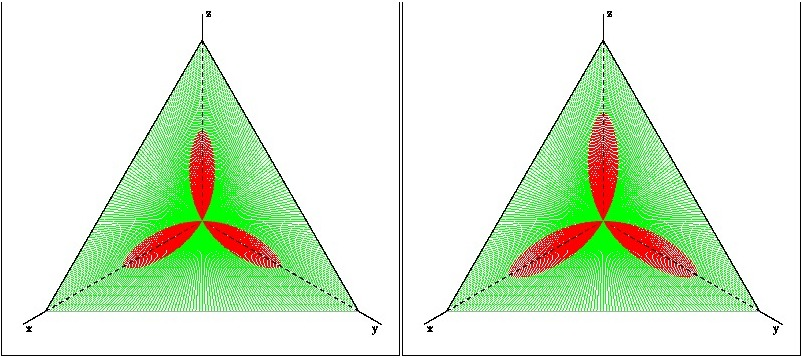
\includegraphics[width=\textwidth]{fleur-concat.png}
      \caption{\footnotesize These two diagrams illustrate
        inequalities (\ref{eq:iengaech}) and (\ref{eq:feovaivo}). The
        former displays all points in red which violate
        \textsc{collinear horizon}, measured from the centre. The
        latter displays points in different colours whose orientation
        of asymmetry differs, measured from the centre. The two red
        sets are not the same, but there appears to be a relationship,
        one that ultimately I suspect to be due to the more basic
        property of asymmetry.}
      \label{fig:eeghoomo}
    \end{minipage}
  \end{flushright}
\end{figure}

It is opaque what motivates information theory not only to put
probability distributions farther apart near the periphery, as I would
expect, but also near the centre. I lack the epistemic intuition
reflected in the behaviour. The next subsection on asymmetry deals
with this lack of epistemic intuition writ large.

\subsection{Transitivity of Asymmetry}
\label{subsec:Asymmetry}

Recall Joyce's two axioms Weak Convexity and Symmetry (see page
\pageref{quot:weakconv}). The geometry of reason (certainly in its
Euclidean form) mandates Weak Convexity because the bisector of an
isosceles triangle is always shorter than the isosceles sides. Weak
Convexity also holds for information theory (see appendix
\ref{app:wcs} for a proof). Symmetry, however, fails for information
theory. Fortunately, although I do not pursue this any further here,
information theory arrives at many of Joyce's results even without the
violated axiom.

Asymmetry presents a problem for the geometry of reason as well as for
information theory. For the geometry of reason, the problem is akin to
\textsc{continuity}. For information theory, the problem is the
non-trivial nature of the asymmetries it induces, which somehow need
to be reconnected to epistemic justification. I will consider this
problem in a moment, but first I will have a look at the problem for
the geometry of reason.

Extreme probabilities are special and create asymmetries in updating:
moving in direction from certainty to uncertainty is asymmetrical to
moving in direction from uncertainty to certainty. Geometry of
reason's metric topology, however, allows for no asymmetries.

\begin{quotex}
  \beispiel{Extreme Asymmetry}\label{ex:extreme} Consider two cases
  where for case 1 the prior probabilities are $Y_{1}=(0.4,0.3,0.3)$
  and the posterior probabilities are $Y_{1}'=(0,0.5,0.5)$; for case 2
  the prior probabilities are reversed, so $Y_{2}=(0,0.5,0.5)$ and the
  posterior probabilities $Y_{2}'=(0.4,0.3,0.3)$.
\end{quotex}

Case 1 is a straightforward application of standard conditioning. Case
2 is more complicated: what does it take to raise a prior probability
of zero to a positive number? In terms of information theory, the
information required is infinite. Case 2 is also not compatible with
standard conditioning (at least not with what Alan H{\'a}jek calls the
ratio analysis of conditional probability, see \scite{7}{hajek03}{}).
The geometry of reason may want to solve this problem by signing on to
a version of regularity, but then it violates \textsc{regularity}.
Happy kids, clean house, sanity: the hapless homemaker must pick two.
The third remains elusive. Continuity, a consistent view of
regularity, and symmetry: the hapless geometer of reason cannot have
it all.

Now turn to the woes of the information theorist. Given the asymmetric
similarity measure of probability distributions that information
theory requires (the Kullback-Leibler divergence), a prior probability
distribution $P$ may be closer to a posterior probability distribution
$Q$ than $Q$ is to $P$ if their roles (prior-posterior) are reversed.
That is just what we would expect. The problem is that there is
another posterior probability distribution $R$ where the situation is
just the opposite: prior $P$ is further away from posterior $R$ than
prior $R$ is from posterior $P$. And whether a probability
distribution different from $P$ is of the $Q$-type or of the $R$-type
escapes any epistemic intuition.

For simplicity, let us consider probability distributions and their
associated credence functions on an event space with three mutually
exclusive atoms $\Omega=\{\omega_{1},\omega_{2},\omega_{3}\}$. The
simplex $\mathbb{S}^{2}$ represents all of these probability
distributions. Every point $p$ in $\mathbb{S}^{2}$ representing a
probability distribution $P$ induces a partition on $\mathbb{S}^{2}$
into points that are symmetric to $p$, positively skew-symmetric to
$p$, and negatively skew-symmetric to $p$ given the topology of
information theory.

In other words, if

\begin{equation}
  \label{eq:sksy}
  \Delta_{P}(P')=D_{\mbox{\tiny KL}}(P',P)-D_{\mbox{\tiny KL}}(P,P'),
\end{equation}

then, holding $P$ fixed, $\mathbb{S}^{2}$ is partitioned into three
regions, 

\begin{equation}
  \label{eq:sieruxis}
  \Delta^{-1}(\mathbb{R}_{>0})\hspace{.5in}\Delta^{-1}(\mathbb{R}_{<0})\hspace{.5in}\Delta^{-1}(\{0\})
\end{equation}

One could have a simple epistemic intuition such as \qnull{it takes
  less to update from a more uncertain probability distribution to a
  more certain probability distribution than the reverse direction,}
where the degree of certainty in a probability distribution is
measured by its entropy. This simple intuition accords with what we
said about extreme probabilities and it holds true for the asymmetric
distance measure defined by the Kullback-Leibler divergence in the
two-dimensional case where $\Omega$ has only two elements (see
appendix \ref{app:asytwodims}).

In higher-dimensional cases, however, the tripartite partition
(\ref{eq:sieruxis}) is non-trivial---some probability distributions
are of the $Q$-type, some are of the $R$-type, and it is difficult to
think of an epistemic distinction between them that does not already
presuppose information theory. See figure \ref{fig:concat} for
graphical illustration of this point.

On any account of well-behaved and ill-behaved asymmetries, the
Kullback-Leibler divergence is ill-behaved. Of the four axioms as
listed by Ralph Kopperman for a distance measure $d$ (see
\scite{8}{kopperman88}{89}), the Kullback-Leibler divergence violates
both symmetry and triangularity, making it a \qnull{semi-quasimetric}:

\begin{enumerate}[(m1)]
\item $d(x,x)=0$
\item $d(x,z)\leq{}d(x,y)+d(y,z)$ (triangularity)
\item $d(x,y)=d(y,x)$ (symmetry)
\item $d(x,y)=0$ implies $x=y$ (separation)
\end{enumerate}

The Kullback-Leibler divergence not only violates symmetry and
triangularity, but also \textsc{transitivity of asymmetry}. For a
description of \textsc{transitivity of asymmetry} see \textbf{List B} on page
\pageref{page:listtwo}. For an example of it, consider

\begin{equation}
  \label{eq:transviol}
    P_{1}=\left(\frac{1}{2},\frac{1}{4},\frac{1}{4}\right)  \hspace{.5in}
    P_{2}=\left(\frac{1}{3},\frac{1}{3},\frac{1}{3}\right) \hspace{.5in}
    P_{3}=\left(\frac{2}{5},\frac{2}{5},\frac{1}{5}\right)
\end{equation}

In the terminology of \textsc{transitivity of asymmetry} in \textbf{List B},
$(P_{1},P_{2})$ is asymmetrically positive, and so is $(P_{2},P_{3})$.
The reasonable expectation is that $(P_{1},P_{3})$ is asymmetrically
positive by transitivity, but for the example in (\ref{eq:transviol})
it is asymmetrically negative.

How counterintuitive this is (epistemically and otherwise) is
demonstrated by the fact that in MDS (the multi-dimensional scaling of
distance relationships) almost all asymmetric distance relationships
under consideration are asymmetrically transitive in this sense, for
examples see international trade in \scite{7}{chino78}{}; journal
citation in \scite{7}{coombs64}{}; car switch in
\scite{7}{harshmanetal82}{}; telephone calls in
\scite{7}{harshmanlundy84}{}; interaction or input-output flow in
migration, economic activity, and social mobility in
\scite{7}{coxonetal82}{}; flight time between two cities in
\scite{8}{gentleman06}{191}; mutual intelligibility between Swedish
and Danish in \scite{8}{vanommenetal13}{193}; Tobler's wind model in
\scite{7}{tobler75}{}; and the cyclist lovingly hand-sketched in
\scite{8}{kopperman88}{91}.

This \qnull{ill behaviour} of information theory begs for explanation,
or at least classification (it would help, for example, to know that
all reasonable non-commutative difference measures used for updating
are ill-behaved). Kopperman's objective is primarily to rescue
continuity, uniform continuity, Cauchy sequences, and limits for
topologies induced by difference measures which violate triangularity,
symmetry, and/or separation. Kopperman does not touch axiom (m1),
while in the psychological literature (see especially
\scite{7}{tversky77}{}) self-similarity is an important topic. This is
why an initially promising approach to asymmetric modeling in Hilbert
spaces by Chino (see \scite{7}{chino78}{}; \scite{7}{chino90}{};
\scite{7}{chinoshiraiwa93}{}; and \scite{7}{saburichino08}{}) will not
help us to distinguish well-behaved and ill-behaved asymmetries
between probability distributions. I am explaining the reasons in
appendix \ref{app:eekiquom}.

The failure of Chino's modeling approach to make useful distinctions
among asymmetric distance measures between probability distributions
leads us to the more complex theory of information geometry and
differentiable manifolds. Both the results of Shun-ichi Amari (see
\scite{7}{amari85}{}; and \scite{7}{amarinagaoka00}{}) and Nikolai
Chentsov (see \scite{7}{chentsov82}{}) serve to highlight the special
properties of the Kullback-Leibler divergence, not without elevating
the discussion to a level of mathematical sophistication, however,
where it is difficult to retain the appeal to epistemic intuitions.
Information geometry considers probability distributions as
differentiable manifolds equipped with a Riemannian metric. This
metric, however, is Fisher's information metric, not the
Kullback-Leibler divergence, and it is defined on the tangent space of
the simplex representing finite-dimensional probability distributions.
There is a sense in which the Fisher information metric is the
derivative of the Kullback-Leibler divergence, and so the connection
to epistemic intuitions can be re-established.

For a future research project, it would be lovely either to see
information theory debunked in favour of an alternative geometry (this
paper has demonstrated that this alternative will not be the geometry
of reason); or to see uniqueness results for the Kullback-Leibler
divergence to show that despite its ill behaviour the Kullback-Leibler
is the right asymmetric distance measure on which to base inference
and updating. Chentsov's theory of monotone invariance and Amari's
theory of $\alpha$-connections are potential candidates to provide
such results as well as an epistemic justification for information
theory.

\section{Conclusion}
\label{ascc}

Leitgeb and Pettigrew's reasoning to establish LP conditioning on the
basis of the geometry of reason is valid. Given the failure of LP
conditioning with respect to expectations in \textbf{List A}, it cannot be
sound. The premise to reject is the geometry of reason. A competing
approach, information theory, yields results that fulfill all of these
expectations except \textsc{horizon}. Information theory, however,
fails two other expectations identified in \textbf{List B}---expectations
which the geometry of reason fulfills. I am left with loose ends and
ample opportunity for further work. The epistemic utility approach,
itself a relatively recent phenomenon, needs to come to a deeper
understanding of its relationship with information theory. It is an
open question, for example, if it is possible to provide a complete
axiomatization consistent with information theory to justify
probabilism, standard conditioning, and Jeffrey conditioning from an
epistemic utility approach as Shore and Johnston have done from a
pragmatic utility approach. It is also an open question, given the
results of this paper, if there is hope reconciling information theory
with intuitions we have about epistemic utility and its attendant
quantitative concept of difference for partial beliefs.

\appendix

\section{Appendix: Weak Convexity and Symmetry in Information Geometry}
\label{app:wcs}

Using information theory instead of the geometry of reason, Joyce's
result still stands, vindicating probabilism on epistemic merits
rather than prudential ones: partial beliefs which violate probabilism
are dominated by partial beliefs which obey it, no matter what the
facts are.

Joyce's axioms, however, will need to be reformulated to accommodate
asymmetry. This appendix shows that the axiom Weak Convexity (see
section \ref{eugr}) still holds in information geometry. Consider
three points $Q,R,S\in\mathbb{S}^{n-1}$ (replace $\mathbb{S}^{n-1}$ by the
$n$-dimensional space of non-negative real numbers, if you do not want
to assume probabilism) for which

\begin{equation}
  \label{eq:app1}
  D_{\mbox{\tiny KL}}(Q,R)=D_{\mbox{\tiny KL}}(Q,S).
\end{equation}

I will show something slightly stronger than Weak Convexity: Joyce's
inequality is not only true for the midpoint between $R$ and $S$ but
for all points $\vartheta{}R+(1-\vartheta)S$, as long as
$0\leq\vartheta\leq{}1$. The inequality aimed for is

\begin{equation}
  \label{eq:app2}
  D_{\mbox{\tiny KL}}(Q,\vartheta{}R+(1-\vartheta)S)\leq{}D_{\mbox{\tiny KL}}(Q,R)=D_{\mbox{\tiny KL}}(Q,S).
\end{equation}

To show that it holds I need the log-sum inequality, which is a result
of Jensen's inequality (for a proof of the log-sum inequality see
Theorem 2.7.1 in \scite{8}{coverthomas06}{31}). For non-negative
numbers $a_{1},\ldots,a_{n}$ and $b_{1},\ldots,b_{n}$,

\begin{equation}
  \label{eq:logsum}
  \sum_{i=1}^{n}a_{i}\log\frac{a_{i}}{b_{i}}\geq\left(\sum_{i=1}^{n}a_{i}\right)\log\frac{\sum_{i=1}^{n}a_{i}}{\sum_{i=1}^{n}b_{i}}.
\end{equation}

(\ref{eq:app2}) follows from (\ref{eq:logsum}) via

\begin{align}
  \label{eq:app3}
  &D_{\mbox{\tiny KL}}(Q,R)=\vartheta{}D_{\mbox{\tiny KL}}(Q,R)+(1-\vartheta)D_{\mbox{\tiny KL}}(Q,S)=\notag \\
  &\sum_{i=1}^{n}\left(\vartheta{}q_{i}\log\frac{\vartheta{}q_{i}}{\vartheta{}r_{i}}+(1-\vartheta)q_{i}\log\frac{(1-\vartheta)q_{i}}{(1-\vartheta)s_{i}}\right)\geq\notag \\
  &\sum_{i=1}^{n}q_{i}\log\frac{q_{i}}{\vartheta{}r_{i}+(1-\vartheta)s_{i}}=D_{\mbox{\tiny KL}}(Q,\vartheta{}R+(1-\vartheta)S).
\end{align}

I owe some thanks to physicist friend Thomas Buchberger for help with
this proof. Interested readers can find a more general claim in
Csisz{\'a}r's Lemma 4.1 (see \scite{8}{csiszarshields04}{448}), which
accommodates convexity of the Kullback-Leibler divergence as a special
case.

\section{Appendix: Asymmetry in Two Dimensions}
\label{app:asytwodims}

% See \texttt{http://math.stackexchange.com/questions/1428709/cant-swing-the-proof-for-this-inequality}.

This appendix contains a proof that the threefold partition
(\ref{eq:sieruxis}) of $\mathbb{S}^{1}$ is well-behaved, in contrast
to the threefold partition of $\mathbb{S}^{2}$ as illustrated by
figure \ref{fig:concat}. For the two-dimensional case, i.e.\
considering $p,q\in\mathbb{S}^{1}$ with $0<p,q<1, p+p'=1$ and
$q+q'=1$,

% \begin{align}
%   \label{eq:twodims}
%   \Delta_{q}(p)>0&\mbox{ for }&|p-p'|>|q-q'|\notag \\
%   \Delta_{q}(p)=0&\mbox{ for }&|p-p'|=|q-q'|\notag \\
%   \Delta_{q}(p)<0&\mbox{ for }&|p-p'|<|q-q'|
% \end{align}

\begin{equation}
  \label{eq:twodims}
  \begin{array}{rclcrcl}
  \Delta_{q}(p)&>&0&\mbox{ for }&|p-p'|&>&|q-q'|\\
  \Delta_{q}(p)&=&0&\mbox{ for }&|p-p'|&=&|q-q'|\\
  \Delta_{q}(p)&<&0&\mbox{ for }&|p-p'|&<&|q-q'|
  \end{array}
\end{equation}

where $\Delta_{q}(p)=D_{\mbox{\tiny KL}}(q,p)-D_{\mbox{\tiny
    KL}}(p,q)$ and $D_{\mbox{\tiny
    KL}}(p,q)=p\log\frac{p}{q}+(1-p)\log\frac{1-p}{1-q}$. Part of
information theory's ill behaviour outlined in section
\ref{subsec:Asymmetry} is that in the higher-dimensional case the
partition does not follow the simple rule that higher entropy of $P$
compared to $Q$ implies that $\Delta_{Q}(P)>0$ ($\Delta$ here defined
as in (\ref{eq:sksy})). In the two-dimensional case, however, this
simple rule applies. 

That a comparison in entropy $H(p)=-p\log{}p-(1-p)\log(1-p)$ between
$H(p)$ and $H(q)$ corresponds to a comparison of $|p-p'|$ and $|q-q'|$
is trivial. The proof for (\ref{eq:twodims}) is straightforward given
the following non-trivial lemma establishing a very tight inequality.
Given that $p+p'=1$ and $q+q'=1$ and $p,q,p',q'>0$ it is true
that

\begin{equation}
  \label{eq:lemma}
  \mbox{If }\log(p/q)>\log(q'/p')\mbox{ then }(p+q)\log(p/q)>(p'+q')\log(q'/p')
\end{equation}

Let $x=p/q$ and $y=q'/p'$. I know that $x>y$ since $\log{}x>\log{}y$.
Now I want to show $(p+q)\log{}x>(p'+q')\log{}y$. Note that
$p=xq,q'=p'y,p+q=q(x+1),$ and $p'+q'=p'(y+1)$. Therefore,

\begin{equation}
  \label{eq:thirteena}
  q=\frac{1-y}{1-xy}
\end{equation}

and

\begin{equation}
  \label{eq:thirteenb}
  p'=\frac{1-x}{1-xy}.
\end{equation}

What I want to show is that $x>y$ implies

\begin{equation}
  \label{eq:thirteenc}
  \frac{1-y}{1-xy}(x+1)\log{}x>\frac{1-x}{1-xy}\log{}y.
\end{equation}

Note that $f(x)=(1-x)^{-1}(x+1)\log{}x$ is increasing on $(0,1)$ and
decreasing on $(1,\infty{})$, and consider the following two cases:

(i) When $x<1,y<1$, (\ref{eq:thirteenc}) follows from the fact that
$f$ is increasing on $(0,1)$.

(ii) When $x>1,y>1$, (\ref{eq:thirteenc}) follows from the fact that
$f$ is decreasing on $(1,\infty)$.

Mixed cases such as $x>1,y<1$ do not occur, as for example $x>1$
implies $y>1$.

\begin{figure}[ht]
  \begin{flushright}
    \begin{minipage}[h]{\linewidth}
      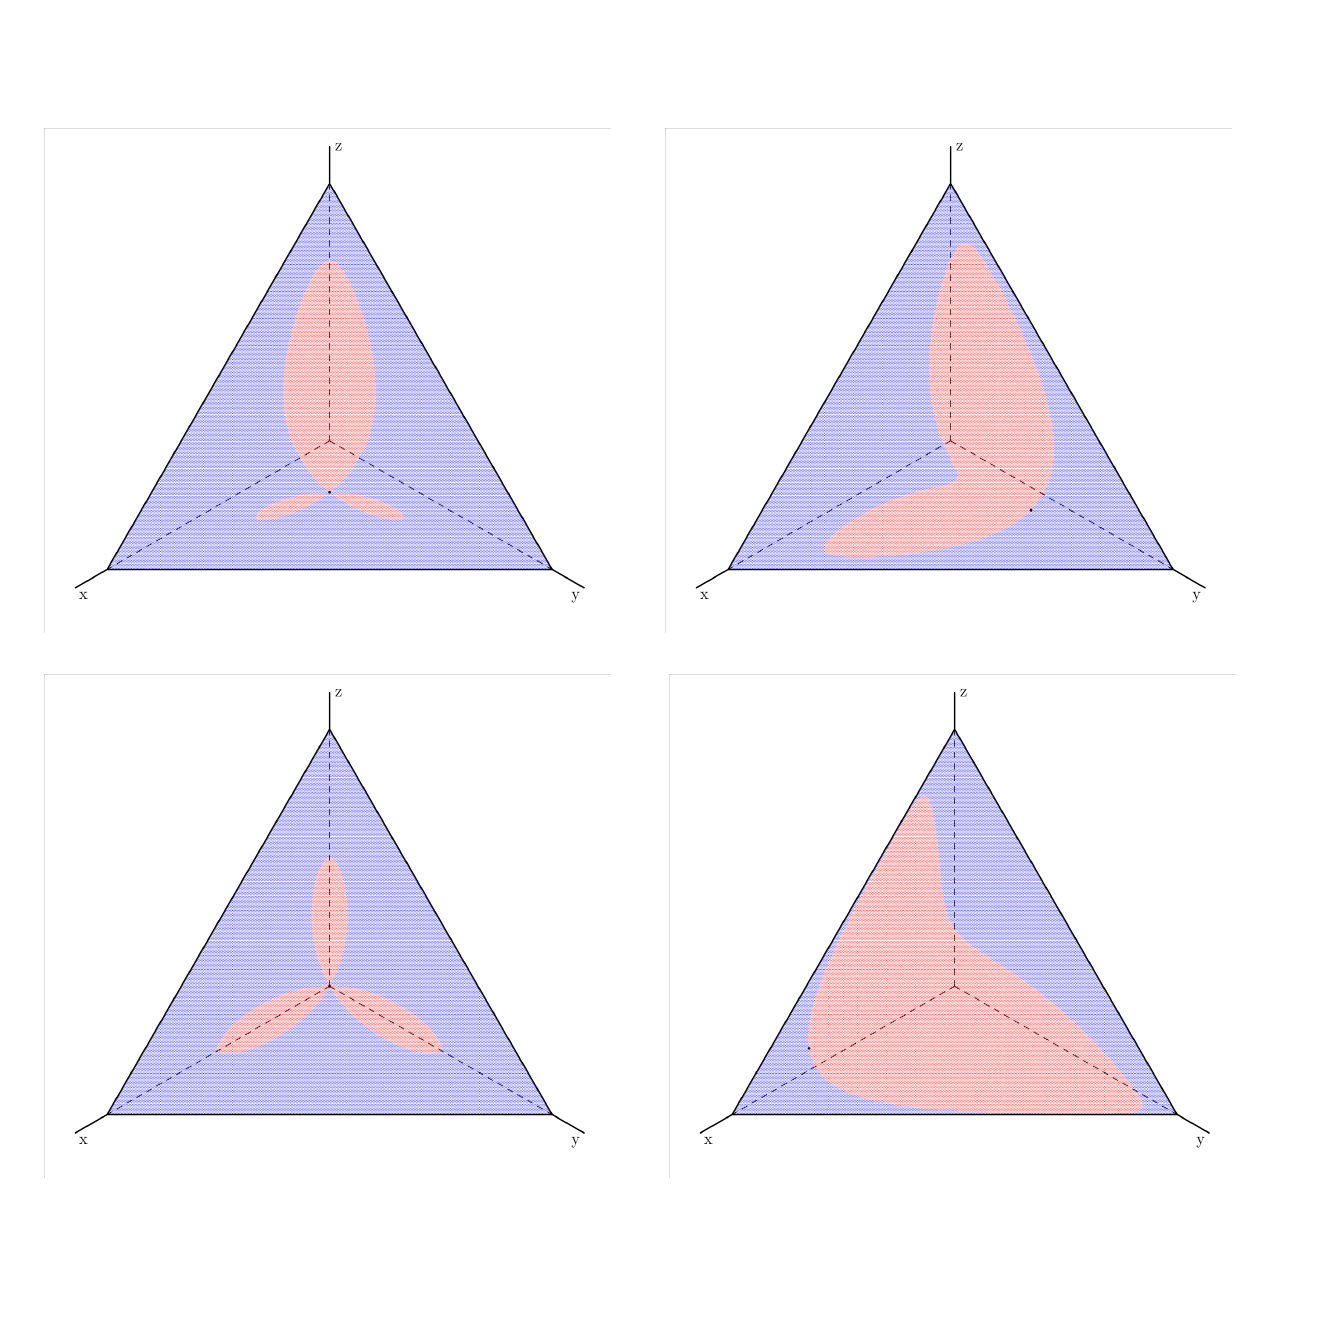
\includegraphics[width=\textwidth]{concat2.png}
      \caption{\footnotesize The partition (\ref{eq:sieruxis}) based
        on different values for $P$. From top left to bottom right,
        $P=(0.4,0.4,0.2); P=(0.242,0.604,0.154); P=(1/3,1/3,1/3);
        P=(0.741,0.087,0.172)$.
        Note that for the geometry of reason, the diagrams are
        trivial. The challenge for information theory is to explain
        the non-triviality of these diagrams epistemically without
        begging the question.}
      \label{fig:concat}
    \end{minipage}
  \end{flushright}
\end{figure}

\section{Appendix: The Horizon Requirement Formalized}
\label{app:horform}

Consider the following two conditions on a difference measure $D$ on a
simplex $\mathbb{S}^{n-1}\subset{}\mathbb{R}^{n}$, which is assumed to
be a smooth function from
$\mathbb{S}^{n-1}\times\mathbb{S}^{n-1}\rightarrow{}\mathbb{R}$.

\begin{enumerate}[(h1)]
\item If $p,p',q,q'$ are collinear with the centre of the
  simplex $m$ (whose coordinates are $m_{i}=1/n$ for all $i$) and an
  arbitrary but fixed boundary point $\xi\in\partial\mathbb{S}^{n-1}$
  and $p,p',q,q'$ are all between $m$ and $\xi$ with
  $\|p'-p\|=\|q'-q\|$ where $p$ is strictly closest to $m$, then
  $|D(p,p')|<|D(q,q')|$. For an illustration of this condition see
  figure \ref{fig:conditions}.
\item Let $\mu\in(-1,1)$ be fixed and $D_{\mu}$ defined as in
  (\ref{eq:defmu}). Then $dD_{\mu}/dx>0$, where $dD_{\mu}/dx$ is the
  total derivative as $x$ moves towards $\xi(x)$, the unique boundary
  point which is collinear with $x$ and $m$.
\end{enumerate}

To define $D_{\mu}$, the hardest part is to specify the domain. Let
this domain $V(\mu)\subseteq{}\mathbb{S}^{n-1}$ be defined as

\begin{equation}
  \label{eq:defvmu}
  V(\mu)=\left\{\begin{array}{ll}
    \{x\in\mathbb{S}^{n-1}|x_{i}<(1-\mu)\xi_{i}(x)+\mu{}m_{i},i=1,\ldots,n\}&\mbox{ for }\mu>0 \\
    \{x\in\mathbb{S}^{n-1}|x_{i}>(1+\mu)m_{i}-\mu{}\xi_{i}(x),i=1,\ldots,n\}&\mbox{ for }\mu<0.
  \end{array}\right.
\end{equation}

Then $D_{\mu}:V(\mu)\rightarrow{}\mathbb{R}^{+}_{0}$ is defined as

\begin{equation}
  \label{eq:defmu}
  D_{\mu}(x)=|D(x,y(x))|
\end{equation}

where $y_{i}(x)=x_{i}+\mu(\xi_{i}(x)-m_{i})$. Remember that $\xi(x)$
is the unique boundary point which is collinear with $x$ and $m$.
Now for the proof that (h1) and (h2) are equivalent. 

First assume (h1) and the negation of (h2). Since $D$ is smooth, there
must be a $\bar{\mu}$ and two points $x'$ and $x''$ collinear with $m$
and a boundary point $\bar{\xi}$ such that
$D_{\bar{\mu}}(x')\geq{}D_{\bar{\mu}}(x'')$ even though
$\|\bar{\xi}-x''\|<\|\bar{\xi}-x'\|$. If this were not the case,
$D_{\mu}$ would be strictly increasing running towards the boundary
points for all $\mu$ and its total derivative would be strictly
positive so that (h2) follows. Now consider the four points
$x',x'',y',y''$ where $y_{i}'=x_{i}'+\mu(\bar{\xi}_{i}-m_{i})$ and
$y_{i}''=x_{i}''+\mu(\bar{\xi}_{i}-m_{i})$ for $i=1,\ldots,n$. Without
loss of generality, assume $\bar{\mu}>0$. Then $x',x'',y',y''$ fulfill
the conditions in (h1) and $D_{\bar{\mu}}(x')<{}D_{\bar{\mu}}(x'')$,
in contradiction to the aforesaid.

Then assume (h2). Let $x',x'',y',y''$ be four points as in (h1).
Consider $\mu=\|\xi-m\|/\|x''-x'\|$. Then $D_{\mu}(x')=|D(x',x'')|$
and $D_{\mu}(y')=|D(y',y'')|$. (h2) tells us that along a path from
$m$ to $\xi$, $D_{\mu}$ is strictly increasing, so
$D_{\mu}(x')=|D(x',x'')|<|D(y',y'')|=D_{\mu}(y')$. QED.

Note that the Euclidean distance function violates both (h1) and (h2)
in all dimensions. The Kullback-Leibler divergence fulfills them if
$n=2$ but violates them if $n>2$. For $n=2$, this is easily checked by
considering the derivative of the Kullback-Leibler divergence for two
dimensions (use $D_{\varepsilon}$ defined in (\ref{eq:defdhpos}) and
(\ref{eq:defdhneg}) for the two-dimensional case instead of $D_{\mu}$
for the arbitrary-dimensional case). A counterexample to fulfillment
of (h1) and (h2) for $n=3$ is given in (\ref{eq:ubiesohx}).

Now that I have shown that (h1) and (h2) is equivalent, it is easy to
show that $J_{P},L_{P}$ and $Z_{P}$ fulfill the horizon requirement
while $M_{P},R_{P}$ and $G_{P}$ violate it. The following table of
derivatives will do (note that $\varepsilon=y-x$ is fixed while $x$
varies and that these derivatives have to be considered with the
absolute value for the various degree of confirmation functions in
mind). Column 1 is the name of the candidate confirmation function;
column 2 is the function with $x$ and $\varepsilon=y-x$ as arguments;
column 3 is the derivative $\partial{}D(x,\varepsilon)/\partial{}x$ for
$|D(x,\varepsilon)|=D(x,\varepsilon)$. 

\begin{tabular}{|l|l|l|}\hline
  $M_{P}(x,y)$ & $\displaystyle{}\varepsilon$ & $0$ \\ \hline
  $R_{P}(x,y)$ & $\displaystyle{}\log\frac{x+\varepsilon}{x}$ & $\displaystyle{}-\frac{\varepsilon}{(x+\varepsilon)x}$ \\ \hline
  $J_{P}(x,y)$ & $\displaystyle{}\frac{x+\varepsilon}{1-x-\varepsilon}-\frac{x}{1-x}$ & $\displaystyle{}\frac{1}{(1-x-\varepsilon)^{2}}-\frac{1}{(1-x)^{2}}$ \\ \hline
  $L_{P}(x,y)$ & $\displaystyle{}\log\frac{(x+\varepsilon)(1-x)}{x(1-x-\varepsilon)}$ & (\ref{eq:lpder}) \\ \hline
  $G_{P}(x,y)$ & $\displaystyle{}\log\frac{1-x}{1-x-\varepsilon}$ & $\displaystyle{}\frac{h}{(1-x)(1-x-\varepsilon}$ \\ \hline
  $Z_{P}(x,y)$ & $\displaystyle{}\frac{\varepsilon}{1-x}\mbox{ or }\frac{\varepsilon}{x}$ & $\displaystyle{}\frac{\varepsilon}{(1-x)^{2}}\mbox{ or }-\frac{\varepsilon}{x^{2}}$ \\ \hline
\end{tabular}

with

\begin{equation}
  \label{eq:lpder}
  -\frac{{\left({\left(x + \varepsilon\right)} {\left(1 - x\right)} - {\left(1 - x - \varepsilon\right)} x\right)} {\left(1-2x-\varepsilon\right)}}{{\left(x + \varepsilon\right)} {\left(1-x-\varepsilon\right)} {\left(1-x\right)} x}.
\end{equation}

\section{Appendix: The Hermitian Form Model}
\label{app:eekiquom}

Asymmetric MDS is a promising approach to classify asymmetries in
terms of their behaviour. This subsection demonstrates that Chino's
asymmetric MDS, both spatial and non-spatial, fails to give us
explanations for information theory's violation of
\textsc{transitivity of asymmetry}. I am choosing Chino's approach
because it is the most general and most promising of all the different
asymmetric MDS models (see, for example, \scite{7}{chinoshiraiwa93}{},
where Chino manages to subsume many of the other approaches into his
own).

Multi-dimensional scaling (MDS) visualizes similarity of individuals
in data\-sets. Various techniques are used in information visualization,
in particular to display the information contained in a proximity
matrix. When the proximity matrix is asymmetrical, we speak of
asymmetric MDS. These techniques can be spatial (see for example
\scite{7}{chino78}{}), where the proximity relationships are
visualized in two-dimensional or higher-dimensional space; or
non-spatial (see for example \scite{7}{chinoshiraiwa93}{}), where the
proximity relationships are used to identify data sets with abstract
spaces (in Chino's case, finite-dimensional complex Hilbert spaces)
and metrics defined on them.

The spatial approach in two dimensions fails right away for
information theory because it cannot visualize transitivity
violations. The hope for other types of asymmetric MDS is that it
would be able to distinguish between well-behaved and ill-behaved
asymmetries and either exclude or identify better-behaved candidates
than the Kullback-Leibler divergence for measuring the distance
between probability distributions. I will use Chino's most
sophisticated non-spatial account to show that asymmetric MDS cannot
solve this problem. For other asymmetric MDS note that with the
Hermitian Form Model Chino seeks to integrate and generalize over all
the other accounts. 

Assume a finity proximity matrix. I will work with two examples here
to avoid the detailed and abstract account provided by Chino. The
first example is

\begin{equation}
  \label{eq:simpromat}
D=\left[
      \begin{array}{ccc}
        0 & 2 & 3 \\
        3 & 0 & 1 \\
        -1 & 2 & 0 
      \end{array}
\right]
\end{equation}

and allows for easy calculations. The second example corresponds to
(\ref{eq:transviol}), the example for transitivity violation where

\begin{equation}
  \label{eq:dklpromat}
\hat{D}=\left[
      \begin{array}{ccc}
0.0000 &  0.0566 &  0.0487 \\
0.0589 &  0.0000 &  0.0499 \\
0.0437 &  0.0541 &  0.0000
      \end{array}
\right],
\end{equation}

and the elements of the matrix $\hat{d}_{jk}=D_{\mbox{\tiny KL}}(P_{j},P_{k})$.
Note that the diagonal elements are all zero, as no updating is
necessary to keep the probability distribution constant.

Chino first defines a symmetric matrix $S$ and a skew-symmetric matrix
$T$ corresponding to the proximity matrix such that $D=S+T$.

\begin{equation}
  \label{eq:skewsym}
  S=\frac{1}{2}(D+D')\mbox{ and }T=\frac{1}{2}(D-D').
\end{equation}

Note that $D'$ is the transpose of $D$, $S$ is a symmetric matrix, and
$T$ is a skew-symmetric matrix with $t_{jk}=-t_{kj}$. Next we define
the Hermitian matrix

\begin{equation}
  \label{eq:herm}
  H=S+iT,
\end{equation}

where $i$ is the imaginary unit. $H$ is a Hermitian matrix with
$h_{jk}=\overline{h_{kj}}$. Hermitian matrices are the complex
generalization of real symmetric matrices. They have special
properties (see section 8.9 in \scite{7}{antonbusby03}{}) which
guarantee the existence of a unitary matrix $U$ such that

\begin{equation}
  \label{eq:unitary}
  H=U\Lambda{}U^{*},
\end{equation}

where $\Lambda=\mbox{diag}(\lambda_{1},\ldots,\lambda_{n})$ with $n$
the dimension of $D$ and $\lambda_{k}$ the $k$-th eigenvalue of $H$
(theorem 8.9.8 in \scite{7}{antonbusby03}{}). $U$ is the matrix of
eigenvectors with the $k$-th column being the $k$-th eigenvector.
$U^{*}$ is the conjugate transpose of $U$. Given example
(\ref{eq:simpromat}), the numbers look as follows:

\begin{equation}
  \label{eq:simh}
H=\frac{1}{2}\left[
      \begin{array}{ccc}
        0 & 5-i & 2+4i \\
        5+i & 0 & 3-i \\
        2-4i & 3+i & 0 
      \end{array}
\right]
\end{equation}

and

\begin{equation}
  \label{eq:simu}
U=\left[
      \begin{array}{ccc}
   0.019 + 0.639i & -0.375 + 0.195i &  0.514 + 0.386i \\
   0.279 - 0.494i & -0.169 - 0.573i &  0.503 + 0.260i \\
  -0.519 + 0.000i &  0.681 - 0.000i &  0.516 + 0.000i
      \end{array}
\right]
\end{equation}

with $\Lambda=\mbox{diag}(-3.78,0.0715,3.71)$. $\Lambda$ is
calculated using the characteristic polynomial
$\lambda^{3}-14\lambda+1$ of $H$. Notice that the characteristic
polynomial is a depressed cubic (the second coefficient is zero),
which facilitates computation and will in the end spell the failure of
Chino's program for our purposes.

Given example (\ref{eq:dklpromat}), the numbers are
 
\begin{equation}
  \label{eq:dklh}
\hat{H}=\frac{1}{2}\left[
      \begin{array}{ccc}
   0.0000 + 0.0000i &  0.0578 - 0.0011i &  0.046 + 0.003i \\
   0.0578 + 0.0011i &  0.0000 + 0.0000i &  0.052 - 0.002i \\
   0.0462 - 0.0025i &  0.0520 + 0.0021i &  0.000 + 0.000i
      \end{array}
\right]
\end{equation}

and

\begin{equation}
  \label{eq:dklu}
\hat{U}=\left[
      \begin{array}{ccc}
   0.351 - 0.467i & -0.543 + 0.170i & -0.578 - 0.006i \\
  -0.604 + 0.457i & -0.201 - 0.169i & -0.598 + 0.002i \\
   0.290 - 0.000i &  0.779 + 0.000i & -0.555 + 0.000i
      \end{array}
\right]
\end{equation}

with $\Lambda=\mbox{diag}(-0.060,-0.045,0.104)$. 

Chino now elegantly shows how the decomposition of $H=U\Lambda{}U^{*}$
defines a seminorm on a vector space. Let
$\phi(\zeta,\tau)=\zeta\Lambda\tau^{*}$. Then (i)
$\phi(\zeta_{1}+\zeta_{2},\tau)=\phi(\zeta_{1},\tau)+\phi(\zeta_{2},\tau)$,
(ii) $\phi(a\zeta,\tau)=a\phi(\zeta,\tau)$, and (iii)
$\phi(\zeta,\tau)=\overline{\phi(\tau,\zeta)}$. These three conditions
characterize an inner product on a finite-dimensional complex Hilbert
space, but only if a fourth condition is met: positive (or negative)
definiteness ($\phi(\zeta,\zeta)\geq{}0)$ for all $\zeta$). One might
hope that positive definiteness identifies the more well-behaved
asymmetries by associating with them a finite-dimensional complex
Hilbert space with the norm $\|\zeta\|=\sqrt{\phi(\zeta,\zeta)}$
defined on it (Chino himself speculatively mentioned this hope to me
in personal communication).

The hope does not come to fruition. Without a non-trivial
self-similarity relation, all seminorms defined as above are
indefinite, and thus all cats grey in the night. Not only are
well-behaved and ill-behaved asymmetries indistinguishable by the
light of this seminorm, even the seminorms for symmetry are
indefinite. Not only does this not help our programme, it also puts a
serious damper on Chino's, who never mentions the self-similarity
requirement (which, given that we are dealing with a proximity matrix,
is substantial).

Based on a theorem in linear algebra (see theorem 4.4.12 in
\scite{7}{antonbusby03}{}),

\begin{equation}
  \label{eq:linalgtheorem}
    \sum_{j=1}^{n}\lambda_{j}=\mbox{tr}(A)
\end{equation}

whenever the $\lambda_{j}$ are the eigenvalues of $A$. The reader can
easily verify this theorem by noticing that the roots of the
characteristic polynomial add up to the second coefficient (which is
the trace of the original matrix). It is well-known that the
eigenvalues of a Hermitian matrix are real-valued (theorem 8.9.4 in
\scite{7}{antonbusby03}{}), which is an important component for Chino
to define the seminorm $\|\zeta\|$ with the help of $\phi$.
Unfortunately, using (\ref{eq:linalgtheorem}), the eigenvalues are not
only real, but also add up to the trace of $H$, which is zero unless
there is a non-trivial self-similarity relation.

Tversky entertains such self-similarity relations in psychology (see
tbd), and Chino is primarily interested in applications in psychology.
When the eigenvalues add up to zero, however, there will be positive
and negative eigenvalues (unless the whole proximity matrix is the
null-matrix), which renders the seminorm as defined by Chino
indefinite. The Kullback-Leibler divergence is trivial with respect to
self-similarity: $D_{\mbox{\tiny KL}}(P,P)=0$ for all $P$.

% \section{References}
% \label{refs}

% \nocite{*} 
\bibliographystyle{ChicagoReedweb} 
\bibliography{bib-2902}

\end{document}
%}}}

